\chapter{A dialect geography approach}\label{ch:5}

\section{Introduction} \label{5.1}
I discussed, in \chapref{ch:4}, the statistical \isi{probability} of a \isi{mono-dialectal account} of origin for the Sranan45 and the fact that the results of that analysis favoured seven input localities with statistically significant degrees of `not by chance' matching with the Sranan45. These areas are Blagdon, Whitwell, Wedmore, Horsington, Canewdon, Doddinghurst and East Mersea. These results presented me with the possibility that the input for the Sranan45 was from two \isi{regional dialect} groups (see \tabref{Table 5.1}).

\begin{table}
\begin{tabular}{ll}
\lsptoprule 
\textbf{Southern \isi{England} Dialect Group} & \textbf{East and East Anglia Dialect Group}\\
\midrule
\textbf{\underline{Sommersetshire}} & \textbf{\underline{Essex}} \\
Blagdon & Doddinghurst \\
Wedmore & East Mersea \\
Horsington & Horsington \\
\\
\textbf{\underline{Hampshire}} &  \\
Withwell (Isle of White) \\
\lspbottomrule 
\end{tabular}
\caption{Regional distribution of the seven lects of statistical significance}
\label{Table 5.1}
\end{table}

\tabref{Table 5.1} highlights the fact that the input for the Sranan45, based on the results of the statistical analysis presented in \chapref{ch:4}, was possibly a composite dialect whose features originated from localities in the south and in the east and East Anglia regions of \isi{England}. Let us see what the distribution highlighted in \tabref{Table 5.1}, looks like on a map of \isi{England} (see Figure \ref{Map5.1} on following page).

\begin{figure}
\includegraphics[width=\textwidth] {figures/highstatloc.pdf}
% % % \captionsetup{name=Map}%
\caption {Distribution of the 7 localities of high statistical significance} 
\label{Map5.1}
\end{figure}

\section{ Linguistic feature mapping} \label{5.2}
The results of the statistical analysis presented in the previous chapter were disregarded and the \textsc{sed45} data was subjected to the \isi{dialect geography} component of analysis. In so doing, the data was used to create geo-linguistic feature mappings of the forty-five putative input forms across \isi{England}. There were two reasons of using this \isi{dialect geography approach}. First, it was a means by which to disconfirm/confirm the results of the statistical analysis. Second, it helped in addressing another possibility that had to be considered; i.e. that the results of the statistical calculations did not account for all conceivable scenarios pointing to the origin(s) of the putative input for the Sranan45 input. To this end, it was hypothesised that the Sranan45 putative input from \isi{England} might have come from converged \isi{dialects}, which might or might not have been situated in the same regional geographic space. Consequently, via the \isi{linguistic feature mapping} of the forty-five \isi{putative input etyma} it would be possible to determine whether there were clusters of localities, which might exhibit denser distributions of the putative input forms than that which might be noticed with Blagdon and its surrounding localities in the south of \isi{England}.

This hypothesis of converged \isi{dialects} is referred to the \emph{Regional Input Hypothesis}. This chapter is a presentation of the steps taken to test this hypothesis, the results of this assessment and the degree of corroboration between the conclusions arrived at in comparison to the results of the statistical analysis presented in \chapref{ch:4}.

\section{Assessing the regional input hypothesis}\label{5.3}
The Regional Input Hypothesis, hereafter \textsc{rih}, was as follows: ``the geo-linguistic source in \isi{England}, of the \textsc{sed45} input etyma relevant to the formation of the Sranan45, was possibly a specific region, i.e. North, South, East and East Anglia, and, West and West Midlands, in which there was a core dialect locality of major \isi{linguistic influence}.'' If this were true, then a \isi{geo-linguistic mapping} of the forty-five putative \textsc{sed45} input etyma would reveal a dense regional distribution of localities in close geographic proximity to this core locality. The above divisions of \isi{England} were based on how  \citet{Orton6271} sectionalised \isi{England} for the \textsc{\textsc{sed}} survey.

\section{Dialect mapping}\label{5.4}
The soundness of the \textsc{rih} was assessed by drawing Concentric Circles of 1cm (27 km) apart, on a \textsc{\textsc{sed}}-inspired map of \isi{England}, from the locality in the northern, east and East Anglia, west and West Midlands, and southern regions of \isi{England}, whose \textsc{sed45} (\textsc{ec}) vector demonstrated the highest levels of correspondence with the Sranan45 target vector, within their respective region. These four regions were selected in accordance with the way in which \citet{Orton6271} sectionalised \isi{England} into regions for the Survey of \ili{English} \isi{Dialects}, undertaken between 1950 and 1961 (see \sectref{3.2.2.1}). These localities of high correspondence in the four regions, i.e. north, west and West Midlands, east and East Anglia, and south, were referred to as Start Lects, \textsc{sl} for short. I took as the region of influence for the Sranan45, any region that fulfilled one major criterion, i.e. that this region's distribution of the relevant features produced the smallest outermost circle in which all of the forty-five putative \textsc{sed45} input etyma are found. An additional characteristic of this criterion was that there was no requirement to move outside of the particular region to secure any variant. The localities situated within this circle would therefore be deemed to be the \isi{regional input} source for the Sranan45.

\subsection{Map conventions and approach}\label{5.4.1}
The map of \isi{England} that was used in the \isi{linguistic feature mapping} was created through a \textsc{php} (Hypertext Pre-processor) script, a simple but powerful scripting language used in webpage creation. In an email message, dated February 22, 2010, its creator Dieter Studer explained that he fashioned the base map by copying the outline of the base map in Viereck's  \emph{Computer-Developed Linguistic Atlas of England} \citep{Viereck90}. The localities surveyed in the \textsc{\textsc{sed}} were plotted on the map via the imaging functionality of \textsc{php} using the same x- and y- values from \citet{Viereck90}. Viereck's Computer-Developed Linguistic Atlas of \isi{England}, ``... is the first computer-developed linguistic atlas of \isi{England}... [whose] ... database is that provided by the Survey of \ili{English} \isi{Dialects} ...'' \citep[79]{Viereck97}.

A scale was created for my version of Studer's map, by using the known distance of two locations in \isi{England}, i.e. the distance between Birmingham and London. This is approximately 160.9 km, which is equivalent to 6 cm on the map used in this research. The distance between each 1 cm-apart Concentric Circle drawn on the map is therefore equivalent to approximately 27 km on land.

\subsubsection{Start lects}\label{5.4.1.1}
In each of the four regions of \isi{England} the distribution of the Start Lects
of highest correspondence with the  Sranan45 reflexes were as follows:

\begin{enumerate}
\item {North: Wearhead, Brigham and Wark with \LSfrac{21/45} (47\%);}
\item {West and West Midlands: Hartlebury, Latterbridge, Earl's Croome and
Grenton with \LSfrac{22/45} (49\%);}
\item {East and East Anglia: Doddinghurst, Canewdon and East Mersea with
\LSfrac{23/45} (51\%);}
\item {South: Blagdon with \LSfrac{27/45} (60\%).}
\end{enumerate}

The first three regions, i.e. the north, west and east \& East Anglia of \isi{England}, posed a problem. Several localities in these regions attained the highest regional score, albeit with different combinations of the forty-five \textsc{sed45} \isi{putative input etyma} for the Sranan45. This issue of competing distributions was dealt with by selecting from among the competing localities in each region, the locality that required the smallest circle to include the other competing areas (see Figures~\ref{Map5.2}--\ref{Map5.4}).
 

\begin{figure}
\centering
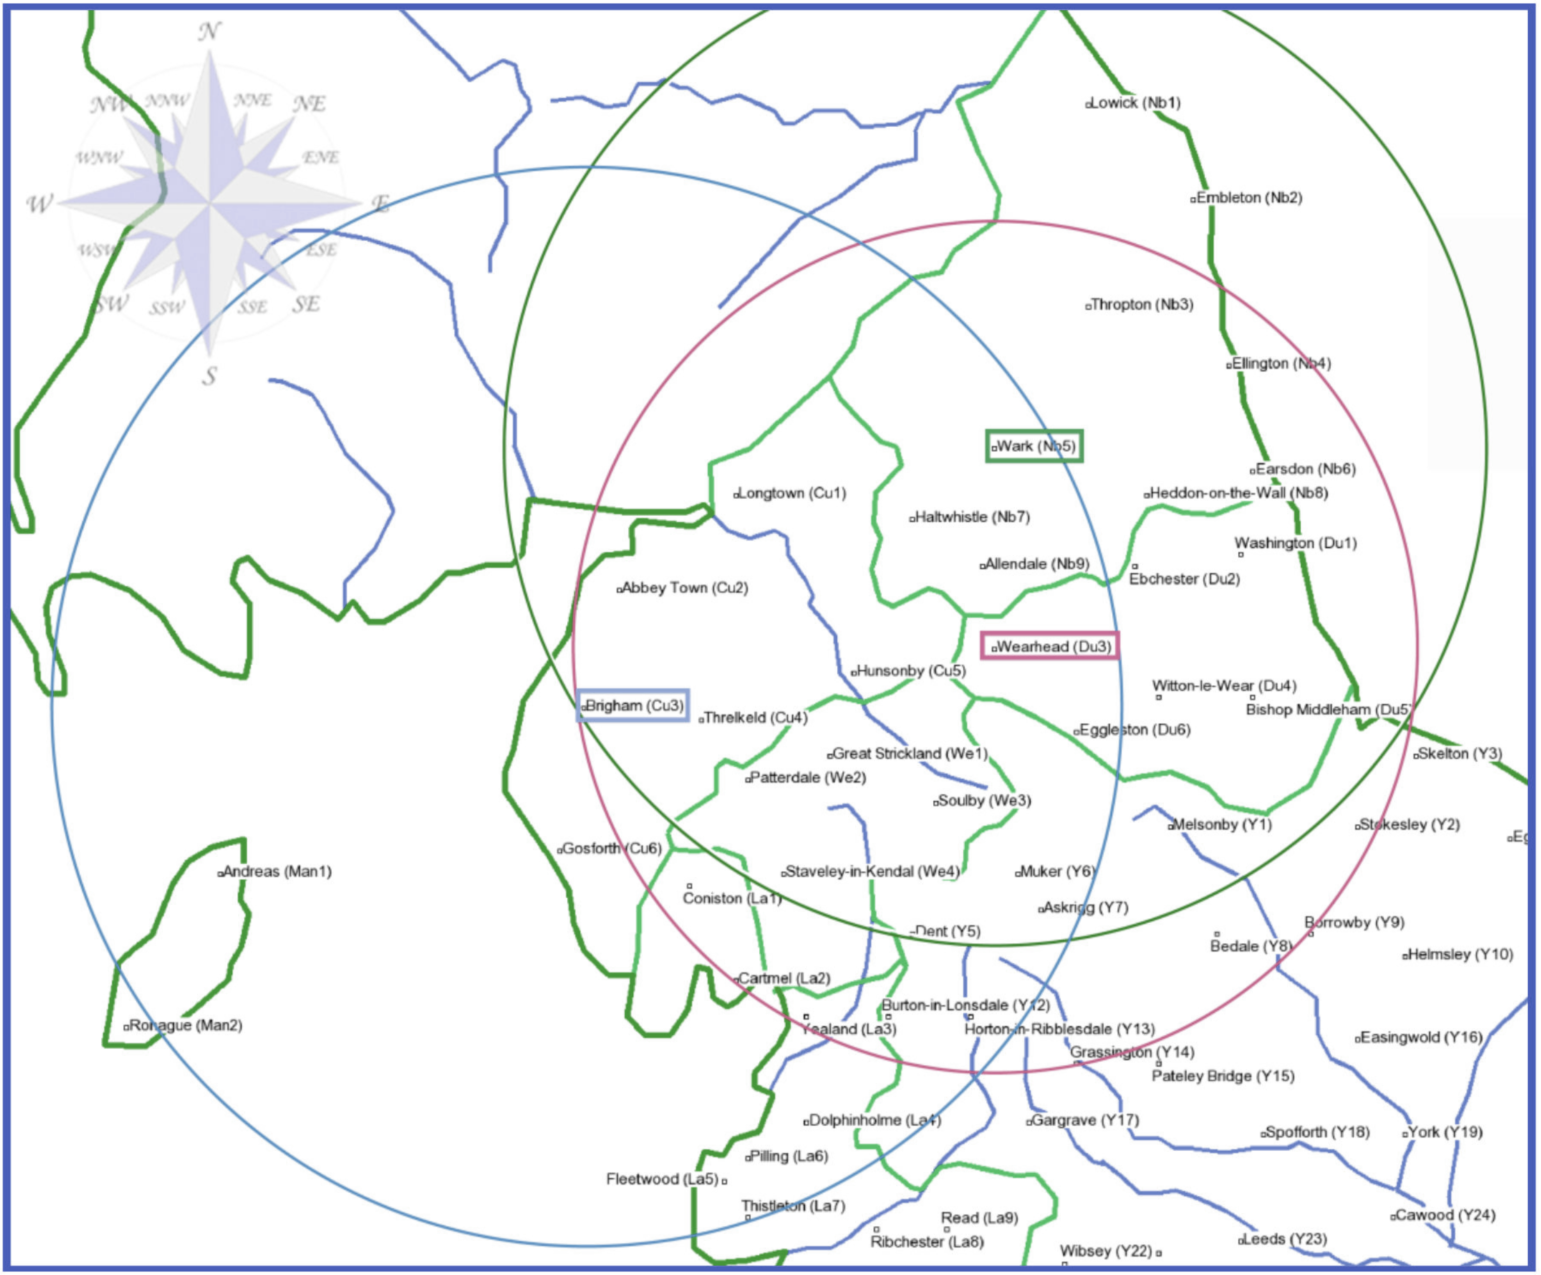
\includegraphics[width=0.98\textwidth] {figures/north-loc.pdf}
% % % \captionsetup{name=Map}%
\caption {Optimal start lect candidate: North of England} 
\label{Map5.2}
\end{figure}


As illustrated in the Figure \ref{Map5.2}, potential \textsc{sl} Wearhead (purple) exhibited the smallest circle in which the other two potential \textsc{sl}s for the north of \isi{England} were captured. Wearhead's radius is 102.06 km (3.78 cm); the other two potential \textsc{sl}s, i.e. Wark and Brigham, have a radius of 121.5 km (4.5 cm) and 135 km (5 cm), respectively.
 

\begin{figure}
\includegraphics[width=0.88\textwidth] {figures/west-loc.pdf}
% % % \captionsetup{name=Map}%
\caption {Optimal start sect candidate: West and West Midlands of England} 
\label{Map5.3}
\end{figure}

\largerpage
As illustrated in the Figure \ref{Map5.3}, potential \textsc{sl} Earl's Croome (purple) exhibited the smallest circle in which the other two potential \textsc{sl} candidates for the west and West Midlands of \isi{England} are captured. Earl's Croome's radius is 110.7 km (4.1 cm); the other two potential \textsc{sl}s, i.e. Hartlebury and Latterbridge, both have a radius of 162 km (6 cm). Let us now look at the optimal \textsc{sl} candidate for the east and East Anglia.
 

\begin{figure}
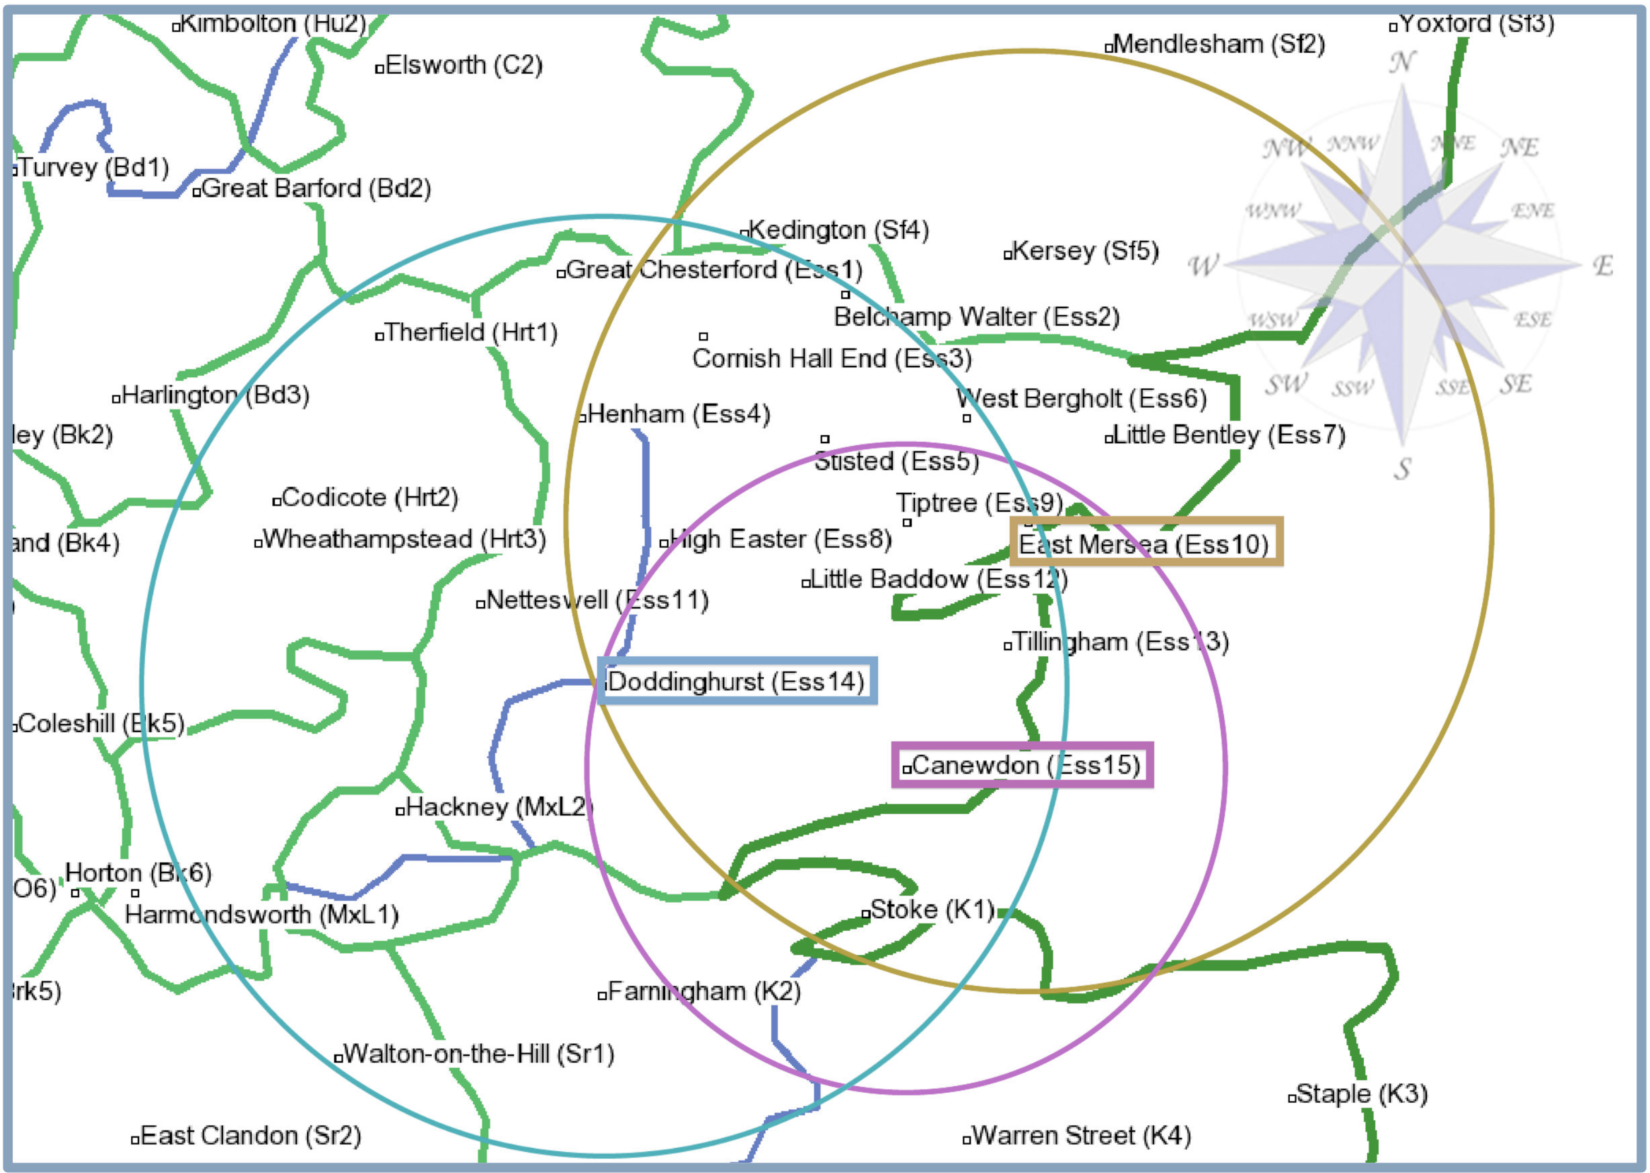
\includegraphics[width=0.98\textwidth] {figures/east-loc.pdf}
% % % \captionsetup{name=Map}%
\caption {Optimal start lect candidate: East and East Anglia of England} 
\label{Map5.4}
\end{figure}

\largerpage
As illustrated in the Figure \ref{Map5.4}, potential \textsc{sl} Canewdon (purple) exhibited the smallest circle in which the other two potential \textsc{sl}s for the east and East Anglia of \isi{England} were captured. Canewdon's radius is 72.9 km (2.7 cm); the other two potential \textsc{sl}s, i.e. Doddinghurst and East Mersea, have a radius of 108 km (4 cm) and 124.2 km (4.6 cm), respectively. This selection process left me with the following \textsc{sl}s:

\begin{enumerate}
\item {North:  \textsc{sl} Wearhead with \LSfrac{21/45};}
\item {West and West Midlands:  \textsc{sl} Earl's Croome with \LSfrac{22/45};}
\item {East and East Anglia:  \textsc{sl} Canewdon with \LSfrac{23/45};}
\item {South:  \textsc{sl} Blagdon with \LSfrac{27/45}.}
\end{enumerate}
 

Having identified these four regional  \textsc{sl}s the next step was to use Concentric Circles of 1 cm (27 km) apart, going outwards from Wearhead in the north, Canewdon in the east and East Anglia, Earl's Croome in the west and Blagdon in the south, until all relevant \textsc{sed45} input variants for the Sranan45 were secured. In taking this approach, I could assess the \isi{pan-dialectal account} of origin, i.e. whether the origin of the Sranan45  input forms originated from all over \isi{England}, as would be the case if \citet{Mufwene08, Mufwene01} ``all over'' account of origin were correct (see \chapref{ch:2}).

The rationale behind this was that if there is a need to cover the same distance outwards from each \textsc{sl}, within its respective region, to secure the relevant input forms, then this would be strong evidence that the input was from all over \isi{England} as opposed to my theorized converged regional \isi{dialects} hypothesis. Consequently, this method of analysis would serve as a means by which to determine whether there were regionally distributed clusters of localities, which exhibited denser distributions of the putative input forms than that which might be noticed with Blagdon and its surrounding localities in the south of \isi{England}.

\section{Map work}
There are two types of maps and one table used to present the distribution of the putative input beginning from each of the four  \textsc{sl}s. These are \emph{Input \isi{Variants} Distribution Maps}, \textsc{\textsc{ivdm}} for short,  \emph{Input \isi{Variants} Route Distribution Maps}, \textsc{ivrdm}, and  \emph{Concentric Circle-by-Concentric Circle Allocation Tables}, hereafter \textsc{ccat}. In the section hereafter, using the data related to the north of \isi{England}, an illustration of how these maps and tables were used to organise and display the data is presented. The presentation of the geo-linguistic data for the three remaining regions follows this.

\subsection{Geo-linguistic distributions}
Beginning with the \textsc{\textsc{ivdm}}s, draw Concentric Circles of 1cm (27 km) apart from each  \textsc{sl}. Continue outwards on the shortest path to the next nearest lect containing an  \textsc{sed45} variant needed for the  Sranan45 target and out again until all the variants are within the circle. Let me illustrate this by presenting the \textsc{\textsc{ivdm}} for the north of \isi{England}.

\begin{figure}
\includegraphics[width=0.95\textwidth] {figures/ivdm1.pdf}
\renewcommand{\thefigure}{\arabic{figure}.5a}
% % % \captionsetup{name=Map}%
\caption{\textsc{ivdm1}: Distribution of remaining putative input items from \textsc{sl} Wearhead (Northern region)} 
\label{Map5.5a}
\end{figure}


The radius of \textsc{sl} Wearhead's distribution is 351 km (13 cm). It seems to span localities in the north, east, west and a portion of the south of \isi{England}. The next step was to highlight using \textsc{ccat}s, the input items found within the Concentric Circles surrounding each  \textsc{sl} and the localities within these circles that exhibited these input forms. A close look at the \textsc{ccat} for the north, i.e. \textsc{ccat1}, highlights the exact \isi{locality-by-locality distribution} of the input items from within the first circle outwards to the final circle (see \textsc{\textsc{ccat}1} (\tabref{Table 5.2})).

\begin{table}
\begin{tabularx}{\textwidth}{lX}
\lsptoprule 
\textbf{Concentric Circle1} & \textbf{arse, broth, corn, remember, turn, care, curse, cold, help, horse, hare} \\
Ebchester (Durham) & [a\textsuperscript{ʁ}ːs], [bʁɒθ], [kɔ\textsuperscript{ʁ}ːn], [ʁɪmɛmbə\textsuperscript{ʁ}], [tɔ\textsuperscript{ʁ}ːn] \\
Allendale (Northumberland) &  [kęə],  [kɔːs] \\
Haltwhistle (Northumberland) & [kɔʊld]   \\
Hunsonby (Cumberland) &   [hɛlp]\\
Soulby (Westmoreland) & [hɑs], [hɛː]  \\
\midrule\textbf{Concentric Circle 2} & \textbf{star, wear, gutter, old} \\
Longtown (Cumberland) & [staːr], [wɛə\textsuperscript{ɹ}] \\
Wark (Northumberland) &  [gʊtʁ], [ɔʊld]\\
\midrule\textbf{Concentric Circle 3} & \textbf{herring}\\
Bedale (Yorkshire) & [jɛɹɪn]  \\
\midrule\textbf{Concentric Circle 5} & \textbf{hear}\\
Leeds (Yorkshire) & [jəɹ] \\
\midrule\textbf{Concentric Circle 8} & \textbf{eyes, woman}\\
Llanymynech (Shropshire) & [haɪz], [wʊmən]  \\
 \midrule\textbf{Concentric Circle 11} & \textbf{yesterday}\\
Longtown (Herefordshire) &  [ɛstə\textsuperscript{ɹ}ɖɪ]\\
\midrule\textbf{Concentric Circle 12} & \textbf{teeth, ears}\\
Harlington (Bedfordshire) & [tiːf]\\
Llanfrechfa (Monmouthshire) & [j\"œs]\\
\midrule\textbf{Concentric Circle 13} & \textbf{ask, mouth}\\
Latterbridge (Gloucestershire) &  [haks] \\
Netteswell (Essex) & [mæʊf]\\
\lspbottomrule 
\end{tabularx}
\caption{\textsc{ccat1}: Wearhead (Durham) \LSfrac{21/45} (24 variants to secure)}
\label{Table 5.2}
\end{table}

Input \isi{Variants} Route Distribution Maps (\textsc{ivrdm})s follow each \textsc{ccat}. \textsc{ivrdm}s are used to depict, based on the information in the \textsc{ccat}s, the locality-to-locality path outwards from each \textsc{sl} to the last locality required to secure all relevant input etyma for the Sranan45 reflexes. On these maps, each \textsc{sl} is highlighted with a star. Take a look at the \textsc{ivrdm} for the north of \isi{England} (see Figure \ref{Map5.5b} on the following page).


\begin{figure}
\includegraphics[width=0.8\textwidth] {figures/ivrdm1.pdf}
\addtocounter{figure}{-1}\renewcommand{\thefigure}{\arabic{figure}.5b}
% % \captionsetup{name=Map}%
\caption {\textsc{ivrdm1}: Distribution path of putative input items from \textsc{sl} Wearhead (Northern Region)} 
\label{Map5.5b}
\end{figure}

With the exception of the divergence to Harlington (Bedfordshire) and Netteswell (Essex) in the east, the distribution of the \textsc{sed45} input forms is in actuality, spread across the north and west of \isi{England} in a line running southwest from Wearhead in the north to Latterbridge in the west. This distribution of the putative input for the Sranan45 is quite dispersed; it is not confined to the north of \isi{England} alone but takes in areas to the west, east and south of \isi{England}. If I noticed a near similar distribution from the other \textsc{sl}, i.e. a distribution that spanned all four regions, I could then have safely assumed that the input for the Sranan45 was from all over \isi{England}. This was not the case however, as will be seen from the presentation of the three remaining regions.

A smaller area of distribution than that noticed from \textsc{sl} Wearhead in the north of \isi{England}, is seen when we move outwards from \textsc{sl} Canewdon in the east of \isi{England}. Take a look at this distribution in \textsc{ivdm2} (Figure \ref{Map5.6a}).

\begin{figure}
\includegraphics[width=\textwidth] {figures/ivdm2.pdf}
\addtocounter{figure}{-1}\renewcommand{\thefigure}{\arabic{figure}.6a}
% % % \captionsetup{name=Map}%
\caption {\textsc{ivdm2}: Distribution of remaining putative input items from \textsc{sl} Canewdon (East and East Anglia region)} 
\label{Map5.6a}
\end{figure}


\textsc{ivdm2} (\ref{Map5.6a}) presents a more concentrated distribution of \textsc{sed45} putative input forms, from \textsc{sl} Canewdon, than that observed for \textsc{sl} Wearhead in the north. The radius of this distribution is 216 km (8 cm), which makes it 135 km (5 cm) smaller than the distribution from \textsc{sl} Wearhead. This distribution of the putative input forms from \textsc{sl} Canewdon seemed to span all localities in the east through to the west and portions of the south of \isi{England}, with no requirement to include any of the localities to the north of \isi{England}. However, \textsc{ccat2} (\tabref{Table 5.3}) told a more precise story concerning the exact nature of this distribution.

\begin{table}
\begin{tabularx}{\textwidth}{lQ}
\lsptoprule 
\textbf{Concentric Circle 1} & \textbf{turn, hare, burn, work} \\  
Tillingham (Essex) & [tə\textsuperscript{ɽ}ːn] \\
Little Baddow (Essex) &  [hɛə] \\
Tiptree (Essex) & [bə\textsuperscript{ɽ}ːn], [wə\textsuperscript{ɽ}ːk]  \\
\midrule
\textbf{Concentric Circle 2} & \textbf{hungry, corn, broth, more (quantity), mouth} \\
Doddinghurst (Essex) & [hʌŋgɹɪ]  \\
Farningham (Kent) &  [gʊtʁ], [kɔ\textsuperscript{ɽ}ːn]\\
Netteswell (Essex) &  [bɹɔ:f], [mɔ\textsuperscript{ə}ɽ], [mæʊf] \\
\midrule
\textbf{Concentric Circle 3} & \textbf{door, more}\\
Great Chesterford (Essex) & [wɛəɹ] \\
\midrule
\textbf{Concentric Circle 4} & \textbf{wear, arse, teeth, star}\\
East Clandon (Surry) & [jəɹ] \\
Harlington (Bedfordshire) & [a\textsuperscript{ɽ}ːs̨] \\
Stewkley (Berkshire) & [stä\textsuperscript{ɽ}] \\
\midrule
\textbf{Concentric Circle 5} & \textbf{yesterday, woman}\\
Tingewick (Berkshire) & [ɪstə\textsuperscript{r}dɪ]  \\
Kislingbury (Northamptonshire) & [wʊmən] \\
\midrule
\textbf{Concentric Circle 6} & \textbf{Hear}\\
Uffington (Berkshire) &  [jɪə\textsuperscript{ɽ}]\\
\midrule
\textbf{Concentric Circle 7} & \textbf{Ask}\\
Latterbridge (Gloucestershire) & [haks]\\
\midrule
\textbf{Concentric Circle 8} & \textbf{ears, eyes}\\
Llanfrechfa (Monmouthshire) &  [j\"œs],  [həɪ]  \\
\lspbottomrule 
\end{tabularx}
\caption{\textsc{ccat2}: Canewdon (Essex) \LSfrac{23/45} (22 variants to secure)}
\label{Table 5.3}
\end{table}

This distribution of the putative input forms follows a path from the east of \isi{England}, with two diversions to Framingham and East Clandon in the south, through the midlands and ends in the west of \isi{England}. This is highlighted in \textsc{ivrdm2} (Figure \ref{5.6b}).


\begin{figure}
\includegraphics[width=\textwidth] {figures/ivrdm2.pdf}
\addtocounter{figure}{-1}\renewcommand{\thefigure}{\arabic{figure}.6b}
% % % \captionsetup{name=Map}%
\caption {\textsc{ivrdm2}: Distribution path of putative input items from \textsc{sl} Canewdon (East and East Anglia region)} 
\label{5.6b}
\end{figure}

The distribution from the west of \isi{England} exhibited an even more concentrated clustering of the putative input forms than that noticed with \textsc{sl} Wearhead and \textsc{sl} Canewdon.
 

\begin{figure}
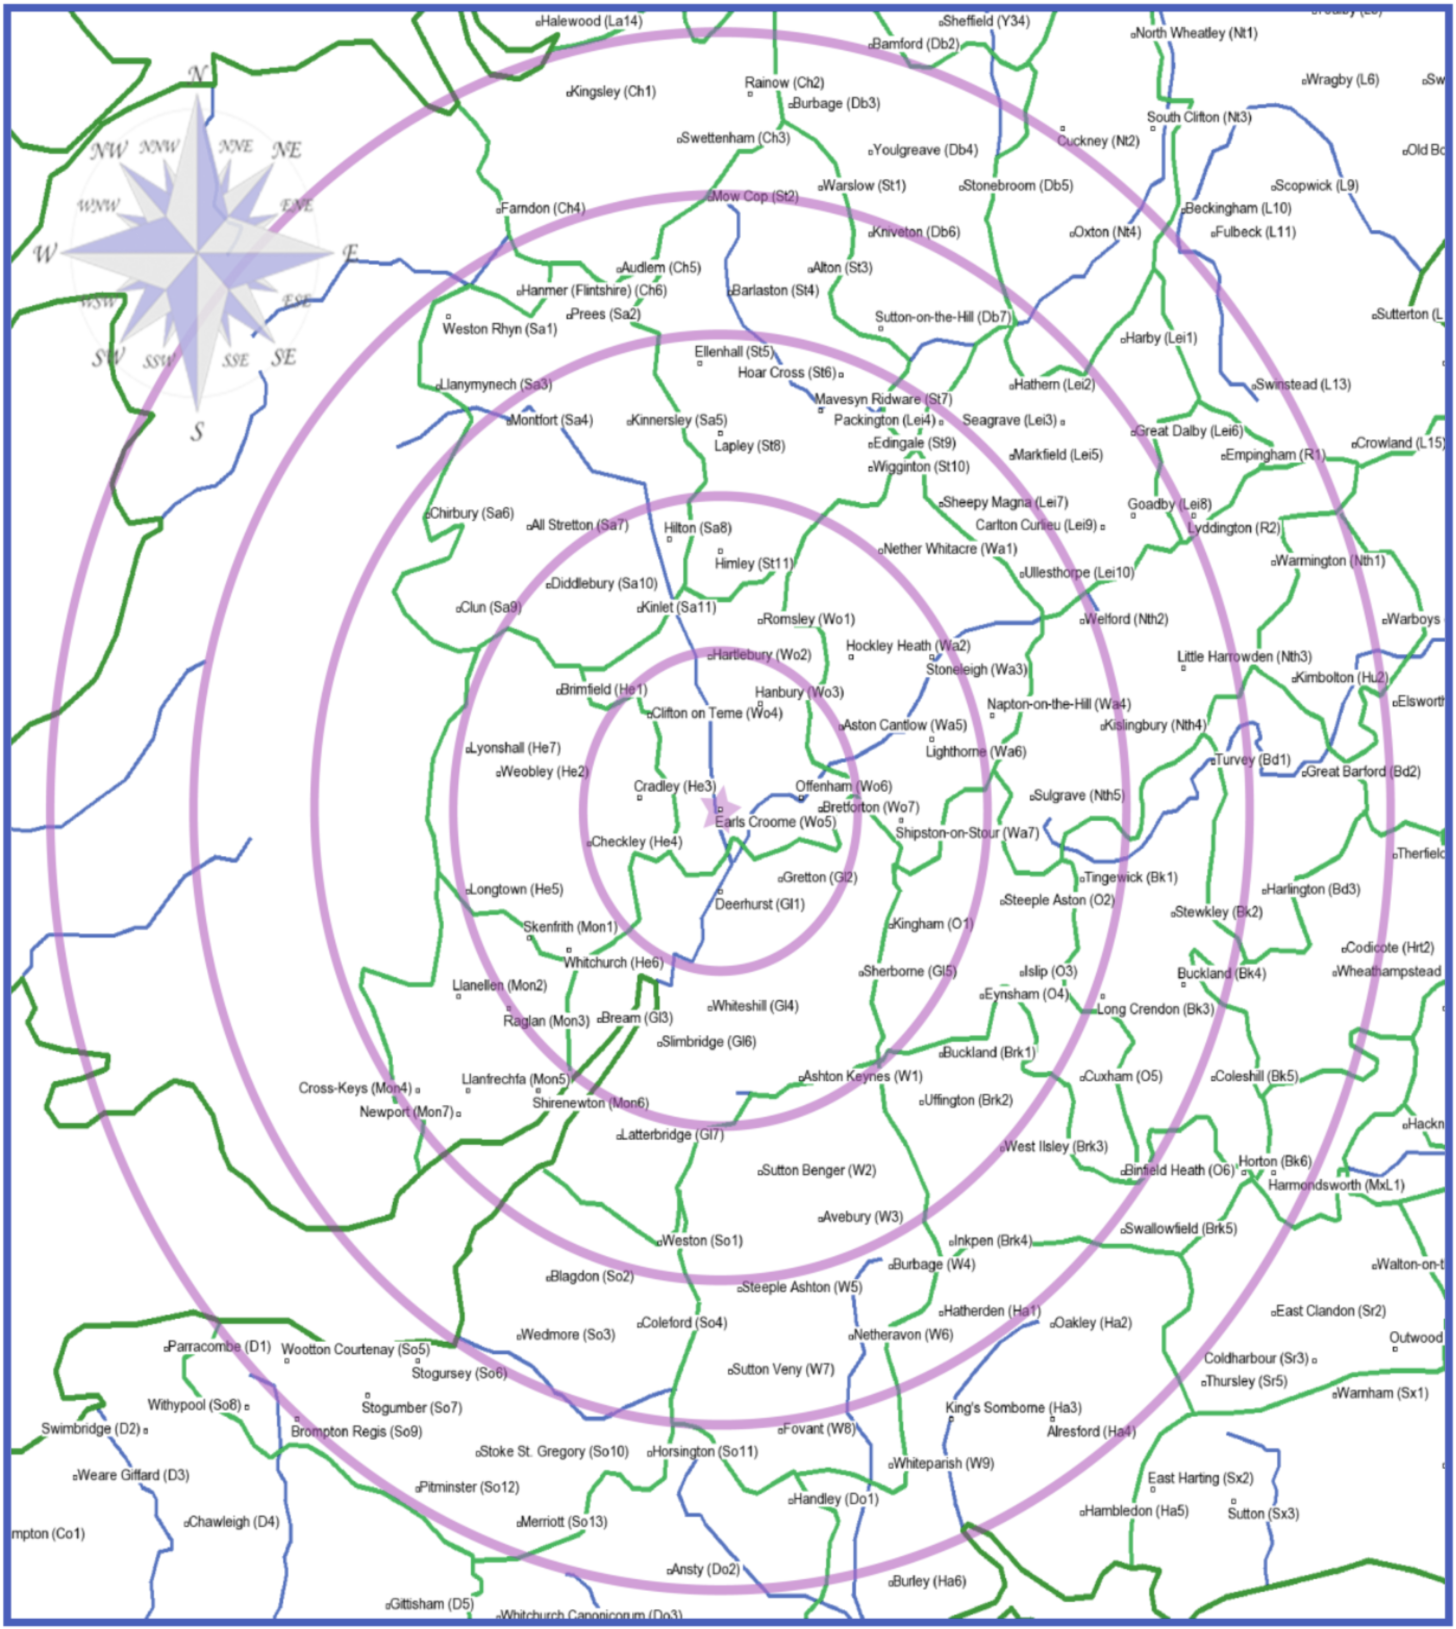
\includegraphics[width=0.9\textwidth] {figures/ivdm3.pdf}
\addtocounter{figure}{-1}\renewcommand{\thefigure}{\arabic{figure}.7a}
% % % \captionsetup{name=Map}%
\caption {\textsc{ivdm3}: Distribution of remaining putative input items from \textsc{sl} Earl's Croome (West and West Midlands region)} 
\label{5.7a}
\end{figure}


The radius of this distribution, from selected \textsc{sl} Earl's Croome, is 135 km (5 cm). This makes it 81 km (3 cm) smaller than that noticed with the distribution from the East \isi{England} \textsc{sl} (Canewdon) and 135 km (5 cm) smaller than that noticed with the distribution from the north \isi{England} \textsc{sl} (Wearhead).


This distribution, as seen in \textsc{ivdm3} (Figure \ref{5.7a}), seems to be concentrated within the west of \isi{England} with a small overlap in the east of \isi{England} and a part of the western section of the south of \isi{England}. Let us take a closer look at the actual locality-by-locality breakdown of the distribution.
 

\begin{table}
\begin{tabularx}{\textwidth}{lX}
\lsptoprule 
\textbf{Concentric Circle 1} & \textbf{finger, brother, yesterday, hog, master (husband)} \\  
Bretforton (Worcestershire) & [fɪŋgə], [bɹʊðə], [ɪstə\textsuperscript{r}dɪ]  \\
Aston Cantlow (Warwickshire) &  [hɑg], [mastə\textsuperscript{ɽ}]  \\
\midrule\textbf{Concentric Circle 2} & \textbf{hot, care, four, hear, gutter} \\
Stoneleigh (Warwickshire) & [hɑt]  \\
Romsley (Worcestershire) &  [keːə]\\
Himley (Staffordshire) &  [fɔ] \\
Skenfrith (Monmouthshire) &  [jə\textsuperscript{r}ɽ] \\
Whiteshill (Gloucestershire) &  [gʊtə\textsuperscript{r}] \\
\midrule\textbf{Concentric Circle 3} & \textbf{ask, hurt, hand, eyes, ears, hungry, fire, house, head}\\
Latterbridge (Gloucestershire) & [haks] \\
Llanfrechfa (Monmouthshire) & [hœt], [hand], [həiz], [jœs], [haŋgɹi] \\
Newport (Monmouthshire) & [faɪə], [həus], [hɛd]  \\
\midrule\textbf{Concentric Circle 4} & \textbf{mouth, help, broth}\\
Blagdon (Somersetshire) & [maʊf], [hɛlp] \\
Wedmore  (Somersetshire) & [brɔf] \\
\midrule\textbf{Concentric Circle 5} & \textbf{teeth}\\
Brompton Regis (Somersetshire) & [tiːf]  \\
\lspbottomrule 
\end{tabularx}
\caption{\textsc{ccat3}: Earl's Croome (Worcestershire) \LSfrac{22/45} (23 variants to secure)}
\label{Table 5.4}
\end{table}

When I transposed this information to an ivrdm, I observed a \isi{geo-linguistic distribution} of input forms concentrated in the west of \isi{England} with an overlap, i.e. a move to localities, in the south of \isi{England}. This overlap covers the southern localities Blagdon, Wedmore and Brompton Regis (see Figure \ref{Map5.7b}).
 

\begin{figure}
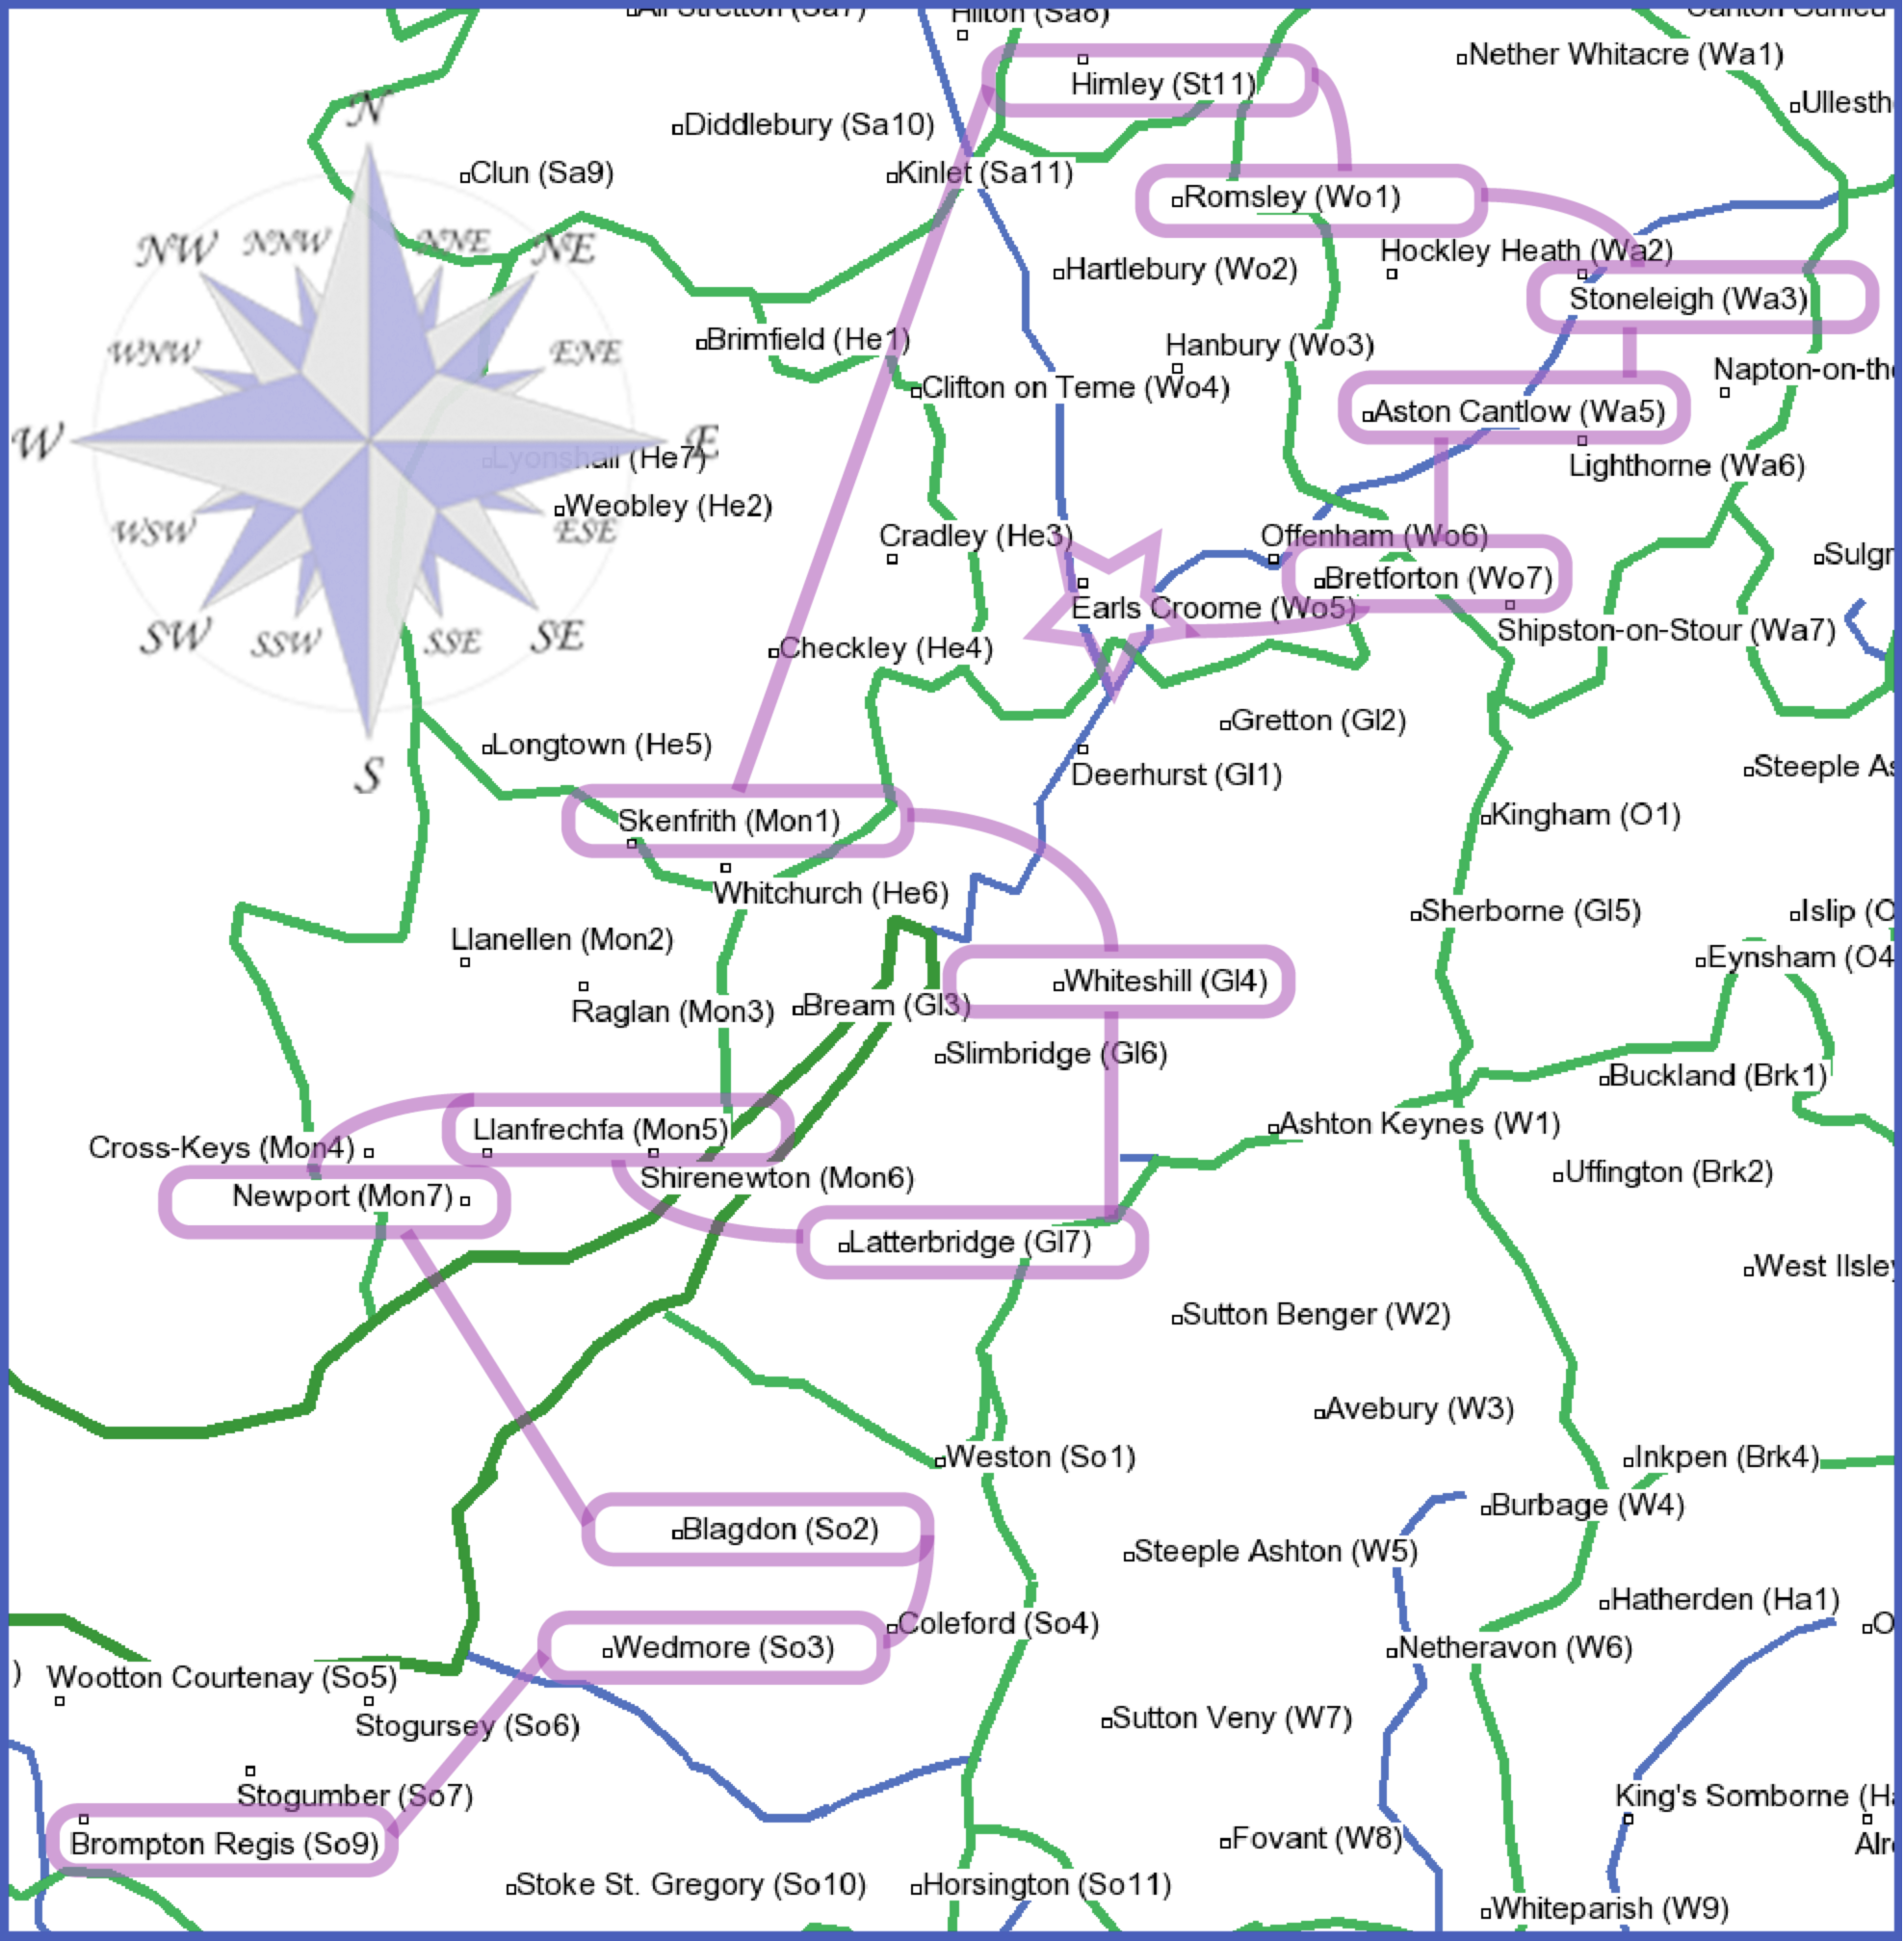
\includegraphics[width=\textwidth,] {figures/ivrdm3.pdf}
\addtocounter{figure}{-1}\renewcommand{\thefigure}{\arabic{figure}.7b}
% % % \captionsetup{name=Map}%
\caption {ivrdm3: Distribution path of putative input items from \textsc{sl} Earl's Croome (West and West Midlands region)} 
\label{Map5.7b}
\end{figure}

In accordance with the pattern thus far, the densest distribution of the input was noticed from the final selected \emph{Start Lect}, Blagdon, in the south of \isi{England} (see the following page).
 

\begin{figure}
\scalebox{0.9}{
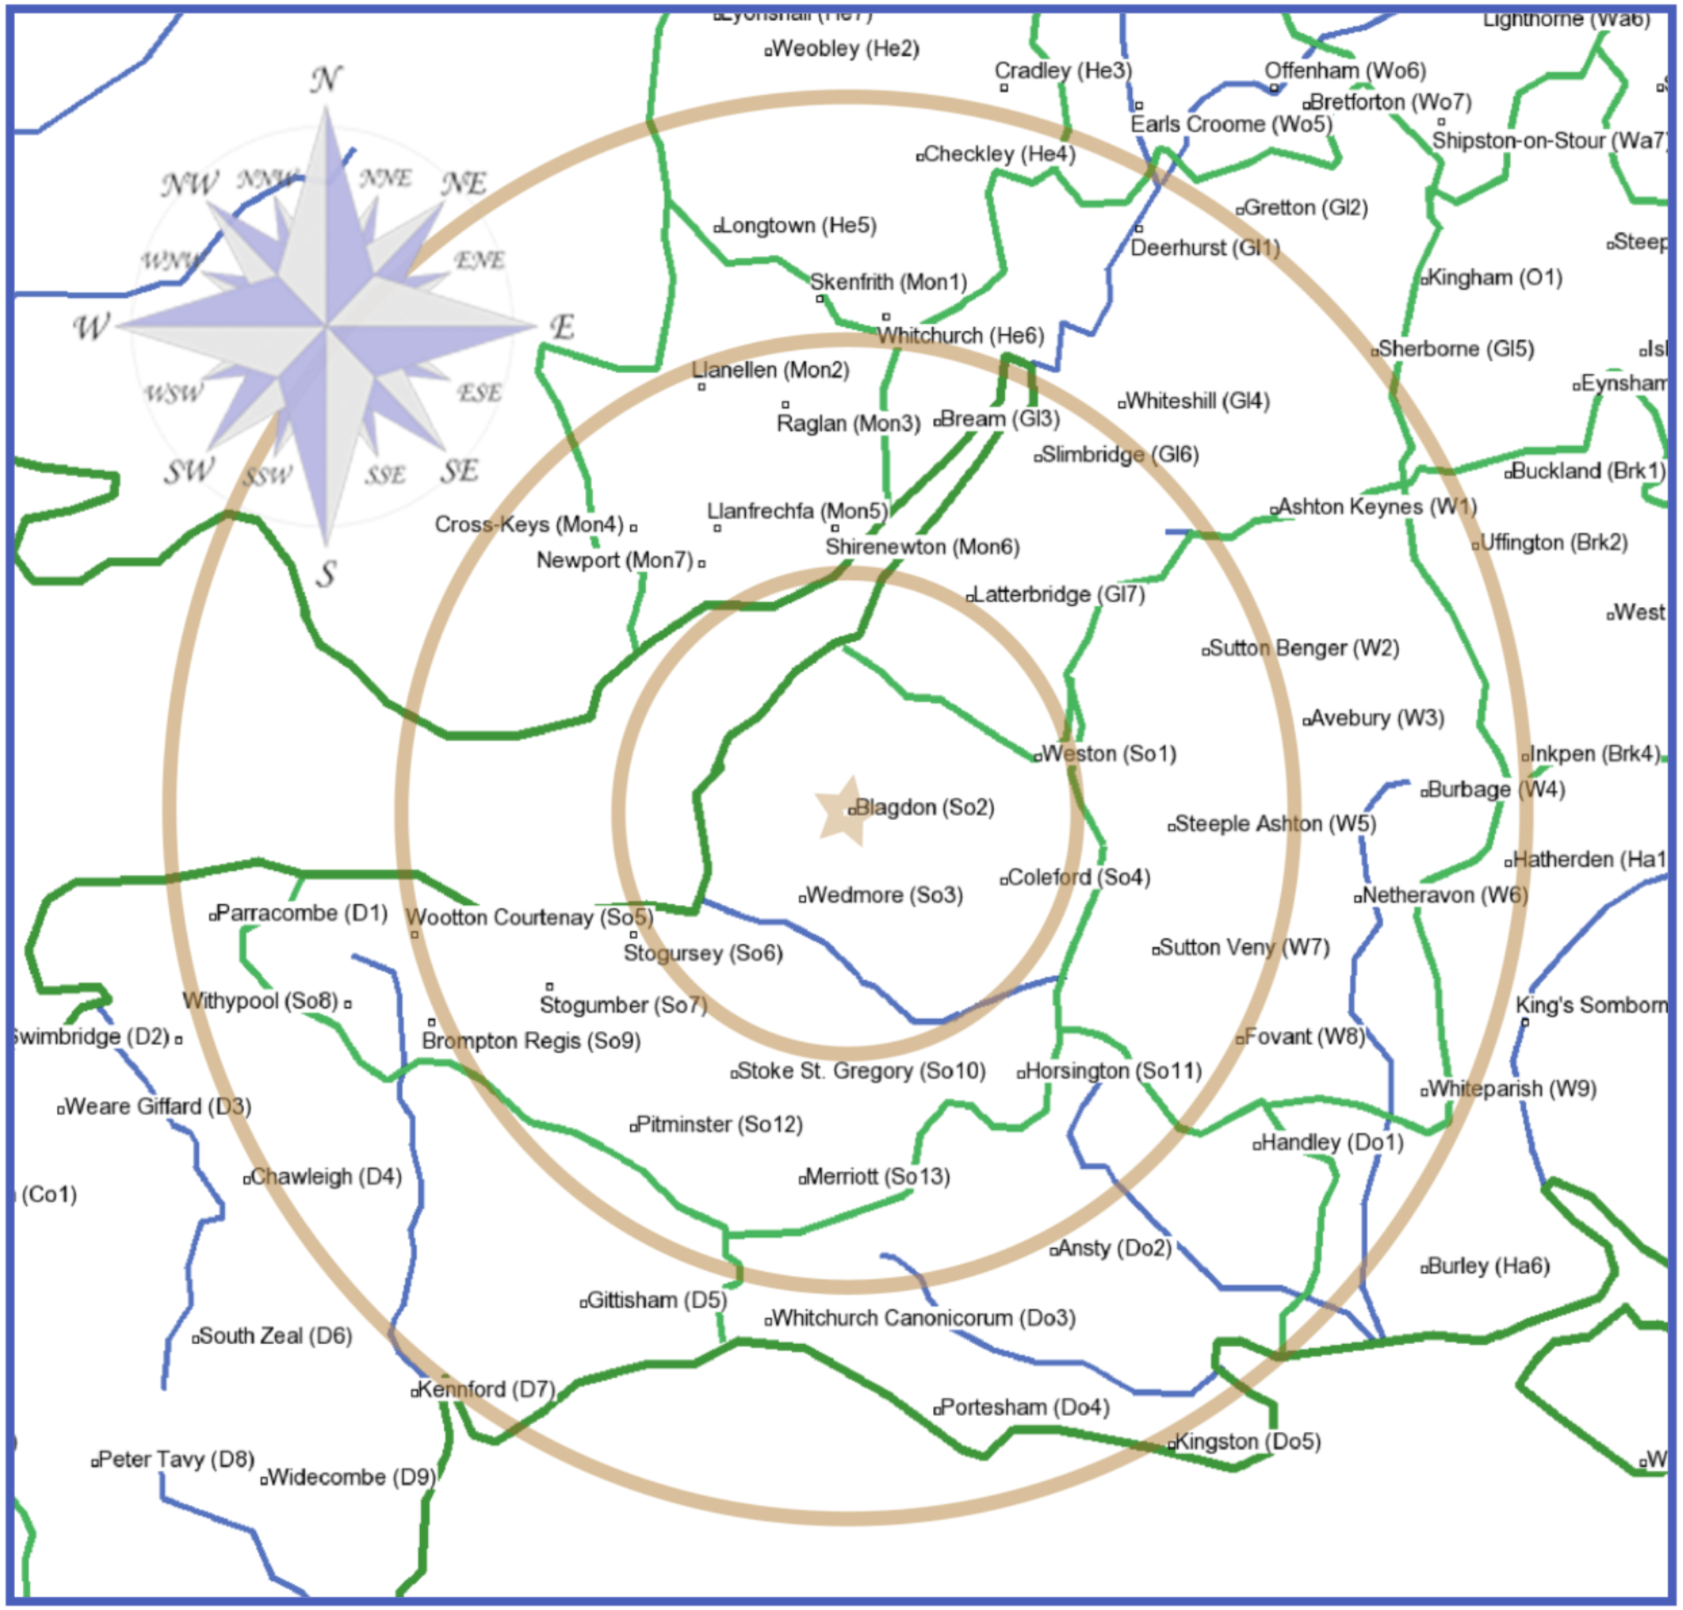
\includegraphics[width=\textwidth] {figures/ivdm4.pdf}
\addtocounter{figure}{-1}\renewcommand{\thefigure}{\arabic{figure}.8a}
% % % \captionsetup{name=Map}%
\caption {\textsc{ivdm4}: Distribution of remaining putative input items from \textsc{sl} Blagdon (Southern region)}
\label{Map5.8a}}
\end{figure}

The radius of the distribution from \textsc{sl} Blagdon is 81 km (3 cm), making this \isi{geo-linguistic distribution} of the putative input forms 54 km (2 cm) smaller than the distribution from the Earl's Croome in the west of \isi{England}, 135 km (5 cm) smaller than the distribution observed from Canewdon in the east of \isi{England} and 270 km (10 cm) smaller than the distribution observed from \textsc{sl} Wearhead in the north of \isi{England}. The \isi{locality-by-locality distribution} of the input variants is as follows:


\begin{table}
\begin{tabularx}{\textwidth}{lX}
\lsptoprule 
\textbf{Concentric Circle 1} & \textbf{broth, hot, hungry, remember, gutter} \\  
Wedmore (Somersetshire) & [bɽɔːf], [hɔt], [hʌŋgɽɪ], [ɽɪmɛmbə\textsuperscript{ɽ}]  \\
Coleford (Somersetshire) &  [gʌtəɽ]  \\
\midrule\textbf{Concentric Circle 2} & \textbf{ask, ears, finger, hurt, brother, care, hare, iron, four arse, eyes} \\
Horsington (Somersetshire) & [a\textsuperscript{ɽ}ːʂ]  \\
Latterbridge (Gloucestershire) &  [haks]\\
Newport (Monmouthshire) &  [j\"œs], [fɪŋgə],  [hœːts]  \\
Llanfrechfa (Monmouthshire) & [b\"{ʌ}ðə], [kɛː], [həɪ], [əɪ-ən], [fɔ]\\
Cross Keys (Monmouthshire) &  [heː\textsuperscript{ə}]\\
\midrule\textbf{Concentric Circle 3} & \textbf{teeth, yesterday}\\ 
Brompton Regis (Somersetshire) & [tiːf] \\
Burbage (Wiltshire) & [estə\textsuperscript{ɽ}ɖeː] \\
\lspbottomrule 
\end{tabularx}
\caption{\textsc{ccat3}: Earl's Croome (Worcestershire) \LSfrac{22/45}  (23 variants to secure)}
\label{Table 5.5}
\end{table}


What \textsc{ccat4} (\tabref{Table 5.5}) highlights is an allocation of the putative \textsc{sed45} input in the most concentrated \isi{geo-linguistic distribution}. All localities in which the relevant linguistic forms are secured, fall into a geographical space characterised by an overlap of the western part of the south of \isi{England}, specifically the counties of Somersetshire and Wiltshire, and, the county of Monmouthshire. Look at Blagdon's ivrdm to get a visual representation of this \isi{locality-by-locality distribution} of the input forms (see the following page).


\begin{figure}
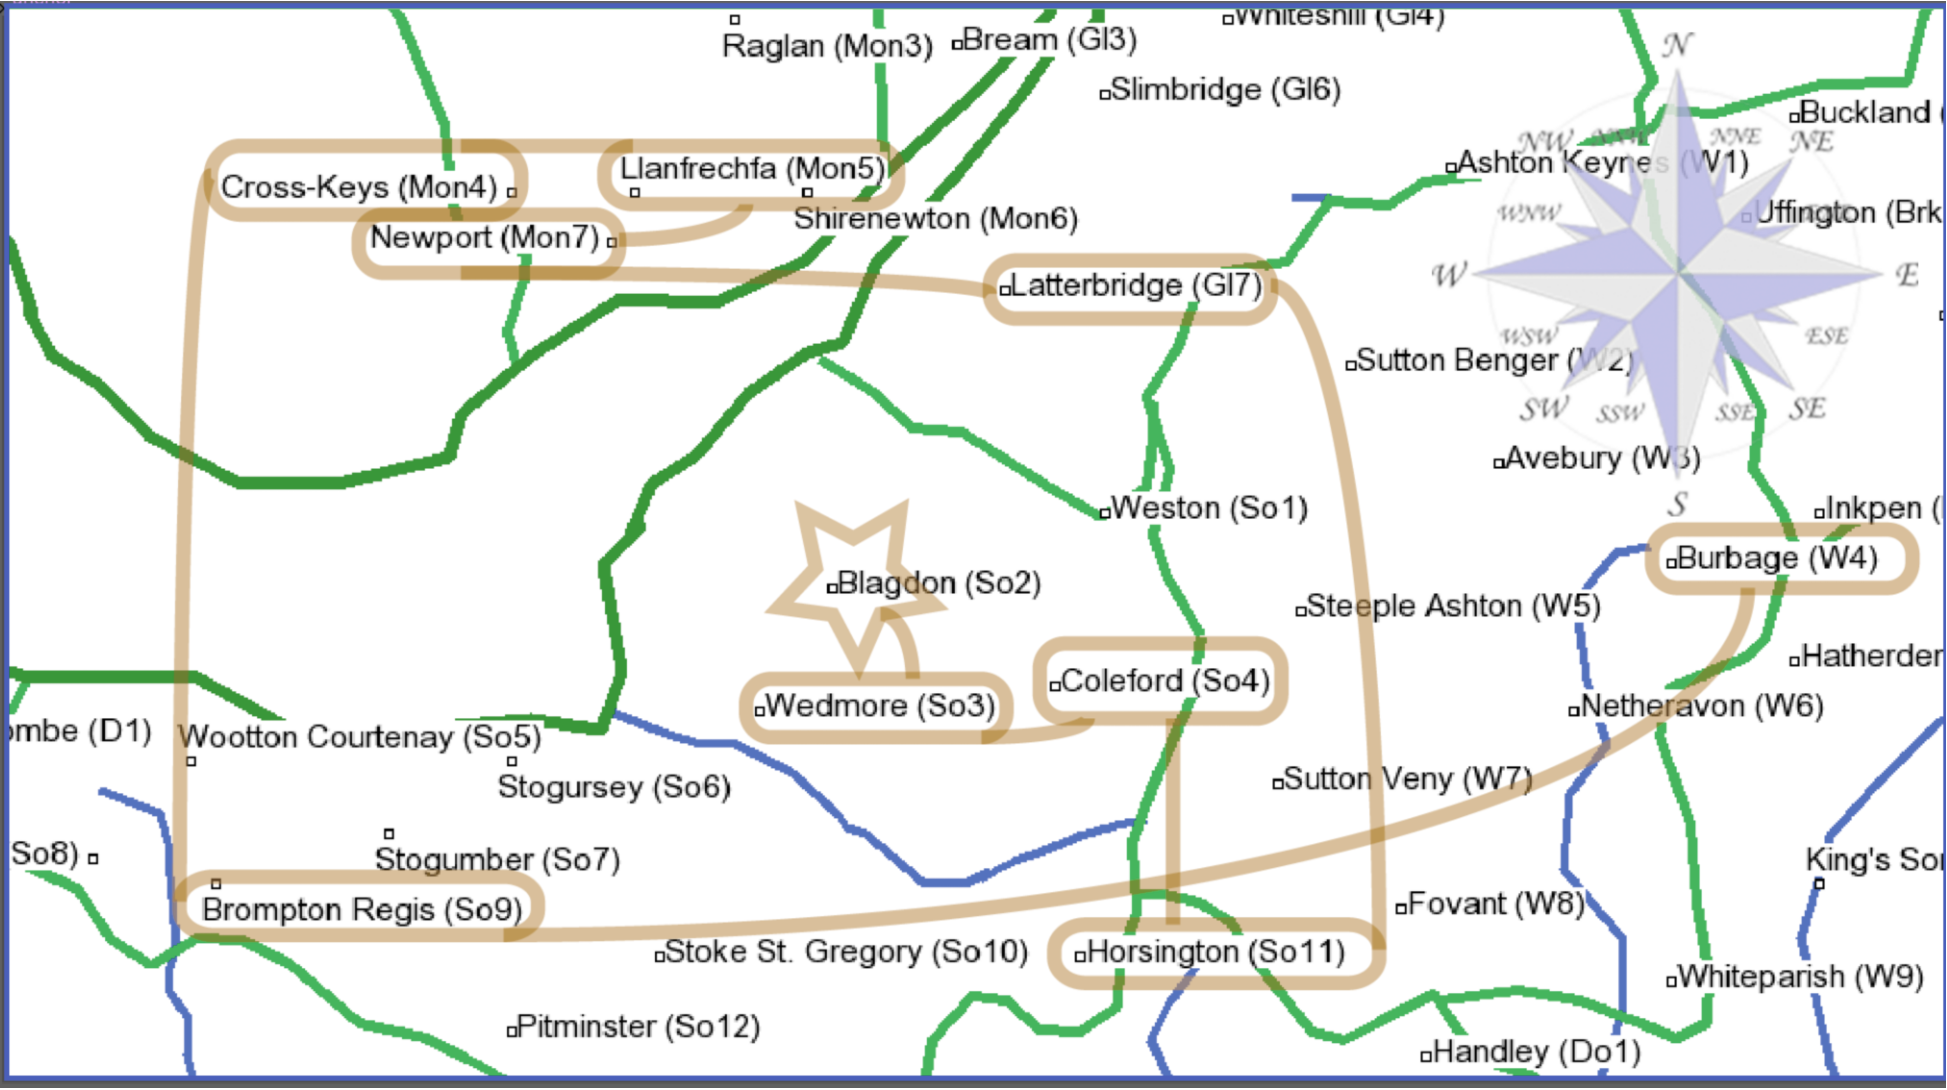
\includegraphics[width=\textwidth, keepaspectratio] {figures/ivrdm4.pdf}
\addtocounter{figure}{-1}\renewcommand{\thefigure}{\arabic{figure}.8b}
% % % \captionsetup{name=Map}%
\caption {\textsc{ivrdm4}: Distribution Path of Putative Input Items from \textsc{sl} Blagdon} 
\label{Map5.8b}
\end{figure}

The distribution presented in Figure \ref{Map5.8b}, represents the most concentrated distribution of the input from \textsc{sl} Blagdon. This distribution spans, in the west-southwest region of \isi{England}, the counties Monmouthshire, Gloucestershire, Somersetshire and Wiltshire. What does all this mean? Let me summarise what these results were saying to me.

\section{What tales do the maps tell?}
Whether I began in \textsc{sl} Wearhead to the north of \isi{England}, \textsc{sl} Canewdon in the east or \textsc{sl} Blagdon to the south, in all cases there was an observed movement towards the localities Llanfrechfa (Monmouthshire) and Latterbridge (Gloucestershire), in the west of \isi{England}, to secure input variants for \emph{eyes } [həɪ] and \emph{ask} [haks], respectively (see Figure \ref{Map5.9}). The Sranan45 reflexes are produced with +/h/ (in this case word initial [h]) and the latter item \emph{ask} is produced with +\textsc{ccr} (consonant cluster reversal), i.e. [hai] and [hakisi], respectively.


\begin{figure}\is{geo-linguistic distribution}
\scalebox{0.8}{
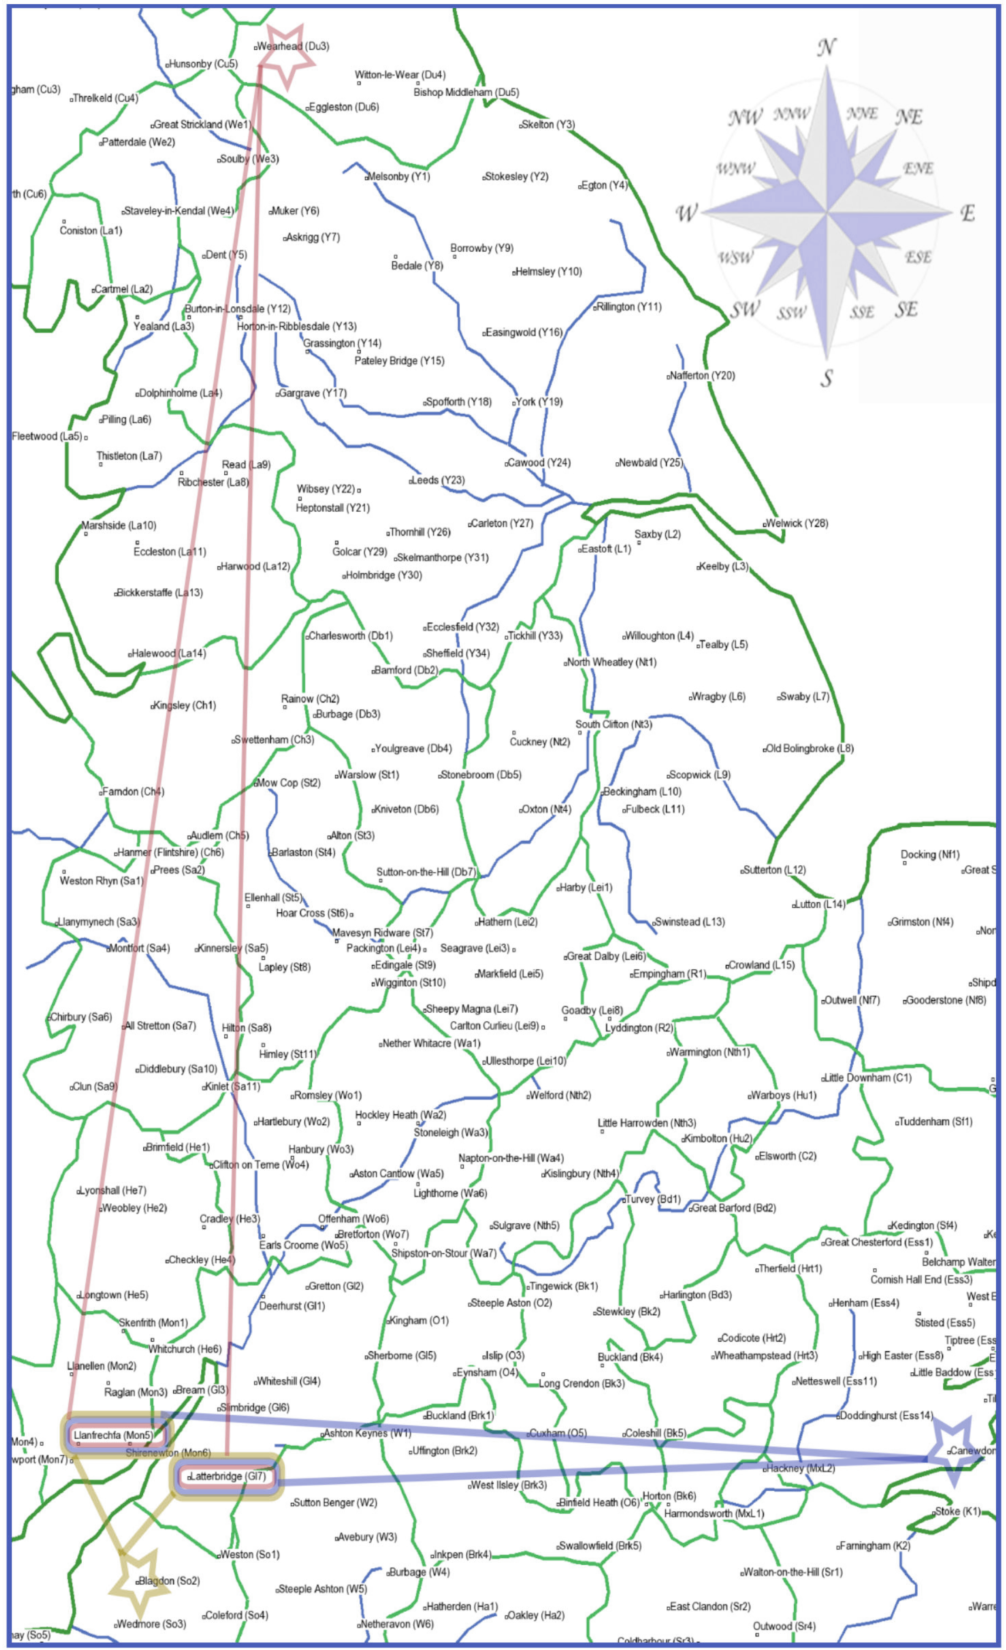
\includegraphics[width=\textwidth] {figures/three-paths.pdf}
\addtocounter{figure}{-1}\renewcommand{\thefigure}{\arabic{figure}.9}
% % % \captionsetup{name=Map}%
\caption {North, West, East: Where three paths of {geo-linguistic distribution} converge}
\label{Map5.9}}
\end{figure}


When I began in \textsc{sl} Earl's Croome in the west of \isi{England}, there was no movement towards the north or east to secure any of the putative \textsc{sed} input etyma for the Sranan45. There was, however, a move to the south of \isi{England}, more specifically in a south-western direction to the county of Somersetshire. The reverse was also true, i.e. when I started in the south of \isi{England}, from \textsc{sl} Blagdon, which is situated within the western end of the southern region, there was a move towards the west of \isi{England} but never to the east or towards the northern region. It is clear from this that the western end of the south of \isi{England} and the west of \isi{England} share a special geo-linguistic relationship.

The \isi{geo-linguistic distribution} of the putative \textsc{sed45} input from Earl's Croome in the west and the distribution from Blagdon in the south comprise of approximately the same localities, i.e. Wedmore, Latterbridge, Llanfrechfa, Newport and Brompton Regis. Added to this, is the fact that the \isi{geo-linguistic distribution} from \textsc{sl} Earl's Croome also includes Blagdon.

The most densely concentrated \isi{geo-linguistic distribution} of the \textsc{sed45} input etyma was observed in an area characterised by an overlap of Orton's west and West Midlands and south \isi{England} regions, specifically the western section of the south. This area, which I refer to as the West Southwest (\textsc{wsw}), comprises of counties: Somersetshire, Monmouthshire, Gloucestershire and Wiltshire. The description \textsc{wsw} is relevant because the \isi{geo-linguistic distribution} of the putative \textsc{sed} input for the Sranan45 was observed halfway between Orton's West and West Midlands region and the western portion of Orton's Southern \isi{England} region. At the centre of this distribution is Blagdon, which like Wedmore, Coleford, Horsington, and Brampton Regis is situated within the \textsc{wsw} county of Somersetshire. I therefore referred to this geo-linguistic cluster of counties, i.e. Somersetshire, together with Wiltshire, Monmouthshire and Gloucestershire as the West Southwest 4, hereafter \textsc{wsw4}.

I, at this point, revisited the results of the statistical analysis presented in \chapref{ch:4} to compare these results with what I had come to know thus far from the geo-\isi{linguistic feature mapping}. The following was apparent to me:

First, Blagdon's status as the most statistically significant core \isi{input dialect} of origin for the Sranan45 was corroborated by the results of the \isi{geo-linguistic mapping}. It is the \textsc{sl} at the core of the densest geo-linguistic concentration of input etyma. Second, Blagdon's 40\% (\LSfrac{18/45}) non-corresponding putative \textsc{sed45} input etyma were found within the dense concentration of localities situated within the \textsc{wsw4} cluster of localities.

Given that there was no need to venture out of the \textsc{wsw4} to secure any of the putative input forms, this strongly suggested that the origin of the Sranan45 was neither from `All-over \isi{England}', nor was it from a single one of Orton et al.'s four broad regions, i.e. northern, east and East Anglia, west and West Midlands or southern \isi{England} \citep{Orton6271}. The area of origin for the Sranan45 input etyma was in fact observed within a small geographic space in \isi{England}. Based on the \isi{linguistic feature mapping} this small geographic space was found to be situated between the southern portion of the west of \isi{England} and the western portion of the south of \isi{England}. The input localities in this small geographic area were observable in four counties that border each other. These are Monmouthshire, Gloucestershire, Wiltshire and Somersetshire; the four counties which together constitute the \textsc{wsw4}.

Furthermore, given the significance of the west of \isi{England}, to which we must travel irrespective of \textsc{sl}, I was presented with another region of input that was not pinpointed by the statistical component of the methodological tool. Although no locality of statistical significance was observed in this region, it was nonetheless a region to which movement must take place to secure the items \emph{ask} and \emph{eyes}, whose lexical and phonetic shapes are peculiar to that region.

In addition, there was no geo-linguistic corroboration for the east \isi{England} input localities presented in \tabref{Table 5.1}. One might want to argue that choice of one of the other two potential \textsc{sl}s, i.e. Doddinghurst or East Mersea, over \textsc{sl} Canewdon, might have resulted in a more concentrated \isi{geo-linguistic distribution} of the input etyma for the Sranan45. This argument can be dispelled based on the fact that whichever of the two (both of which, like Canewdon, are situated in Essex) is taken as the \textsc{sl}, there would still be a need to venture across East Anglia through the West Midlands to localities Llanfrechfa and Latterbridge in the west of \isi{England}, to secure the two items peculiar to those localities, i.e. \emph{ears} with word initial palatal [j] and no \textsc{pvr}, and \emph{ask} with word-initial phonemic /h/ and consonant cluster reversal, /sk/$\rightarrow$[ks].

How then, could the statistical significance of the East \isi{England} lects be explained? If it was only \isi{linguistic feature mapping} that was done and no statistical analysis then the three east and East Anglia lects would not have been pinpointed (see \chapref{ch:7}). Added to this was one other loose end that needed to be addressed. As discussed in \chapref{ch:4}, three other localities to the south of \isi{England} (see \tabref{Table 5.1}), presented themselves as being of near comparable statistical significance with Blagdon. These are: Whitwell \textsc{i.o.w}. in Hampshire County, with a .0078 `not by chance' \isi{probability} of being the \isi{input lect}, and Horsington and Wedmore in Somersetshire County, both with a .0170 `not by chance' \isi{probability} of being the input lects for the Sranan45. The question was, which of the three, if any, might have provided a more credible \textsc{sl}, at the centre of a densely concentrated south \isi{England} source for the Sranan45 input variety?

These loose ends presented me with the challenge of having to explain: (1) all the `not by chance' correspondences being the input source for the Sranan45 and (2) which of the southern \isi{England} lects, i.e. Blagdon, Wedmore, Whitwell and Horsington, provided a more viable candidate for the distribution from the south of \isi{England}. Addressing the first problem would involve an explanation that included all `not by chance' localities constituting the input for the Sranan45; this is dealt with in further detail in \chapref{ch:7}.

Addressing the second problem involved trying to determine from which of the four statistically significant \textsc{wsw} \isi{England} lects I needed to move the shortest distance outwards, in all directions, to secure the relevant \textsc{sed} input for the Sranan45 reflexes. I already presented the distribution of the input from Blagdon. Hereafter I discuss the results arrived at from having plotted the distribution of the remaining putative \textsc{sed} input forms from the three other potential cores for the South, i.e. Whitwell, Horsington and Wedmore.

\begin{figure}

\includegraphics[width=\textwidth]{figures/ivdm5.pdf}
\addtocounter{figure}{-1}\renewcommand{\thefigure}{\arabic{figure}.10}
% % \captionsetup{name=Map}%
\caption {\textsc{ivdm5}: Distribution of putative input items from potential \textsc{sl} Whitwell} 
\label{Map5.10}
\end{figure}


The radius of the \isi{geo-linguistic distribution} of the \isi{putative input etyma} from potential \textsc{sl} Whitwell is 189 km (7 cm). This makes it 108 km (4 cm) larger than Blagdon's. This distribution posed no threat to Blagdon's status of being the nucleus of the \textsc{wsw4} counties, within which the input for the Sranan45 is observed. I nonetheless created Whitwell's \textsc{ccat} (see \textsc{ccat5} (\tabref{Table 5.6})) to see whether the \isi{geo-linguistic distribution} of the putative input forms could add to, or subtract from any of the conclusions presented above.

\begin{table}
\begin{tabularx}{\textwidth}{lQ}
\lsptoprule 
\textbf{Concentric Circle 2} & \textbf{woman, master (husband), four, broth, mouth, teeth, hog, hungry, first} \\  
Alresford (Hampshire) & [wʊmən], [mæːstə\textsuperscript{ɽ}], [fɔ]  \\
Handley (Dorset) & [bɽɔf], [məʊf], [tiːf] \\
Thursley (Surry) & [hɒg], [hʌŋgɹɪ], [fəst] \\
\midrule\textbf{Concentric Circle 3} & \textbf{finger} \\
Coldhabour (Surry) & [fɪŋgə] \\
\midrule\textbf{Concentric Circle 4} & \textbf{brother, care, fire, iron, yesterday}\\
Walton-on-Hill (Surry) & [bɽʌðə], [kɛ], [fɑ], [\,aː\textsuperscript{ə}n] \\
Burbage (Wiltshire) & [eːstə\textsuperscript{ɽ}ɖeː] \\
\midrule\textbf{Concentric Circle 5} & \textbf{ask}\\ 
Latterbridge (Gloucestershire) & [haks] \\
\midrule\textbf{Concentric Circle 7} & \textbf{ears, hurt, eye, hare}\\ 
Newport (Monmouthshire) & [j\"œs], [hœːt] \\
Llanfrechfa (Monmouthshire) & [həɪ]\\
Cross keys (Monmouthshire) & [hɛː\textsuperscript{ə}]\\
\lspbottomrule 
\end{tabularx}
\caption{\textsc{ccat5}: Whitwell (Hampshire) \LSfrac{25/45} (20 variants to secure)}
\label{Table 5.6}
\end{table}

Two observations were readily made about this distribution based on the localities highlighted in \textsc{ccat5} above. First, there is the anticipated movement to the west, to localities Llanfrechfa and Latterbridge, to secure the putative \textsc{sed45} input etyma for \emph{eye} and \emph{ask}, respectively. Second, with the exception of Thursley, Coldharbour and Walton-on-Hill in the county of Surrey, which are located to the eastern end of the south of \isi{England}, the \isi{geo-linguistic distribution} of the \isi{putative input etyma} is observed within and surrounding three of the \textsc{wsw4} counties, i.e. Wiltshire, Monmouthshire and Gloucestershire. Let us now look at the other possibility, i.e. Horsington, which is situated in the county of Somersetshire.


\begin{figure}
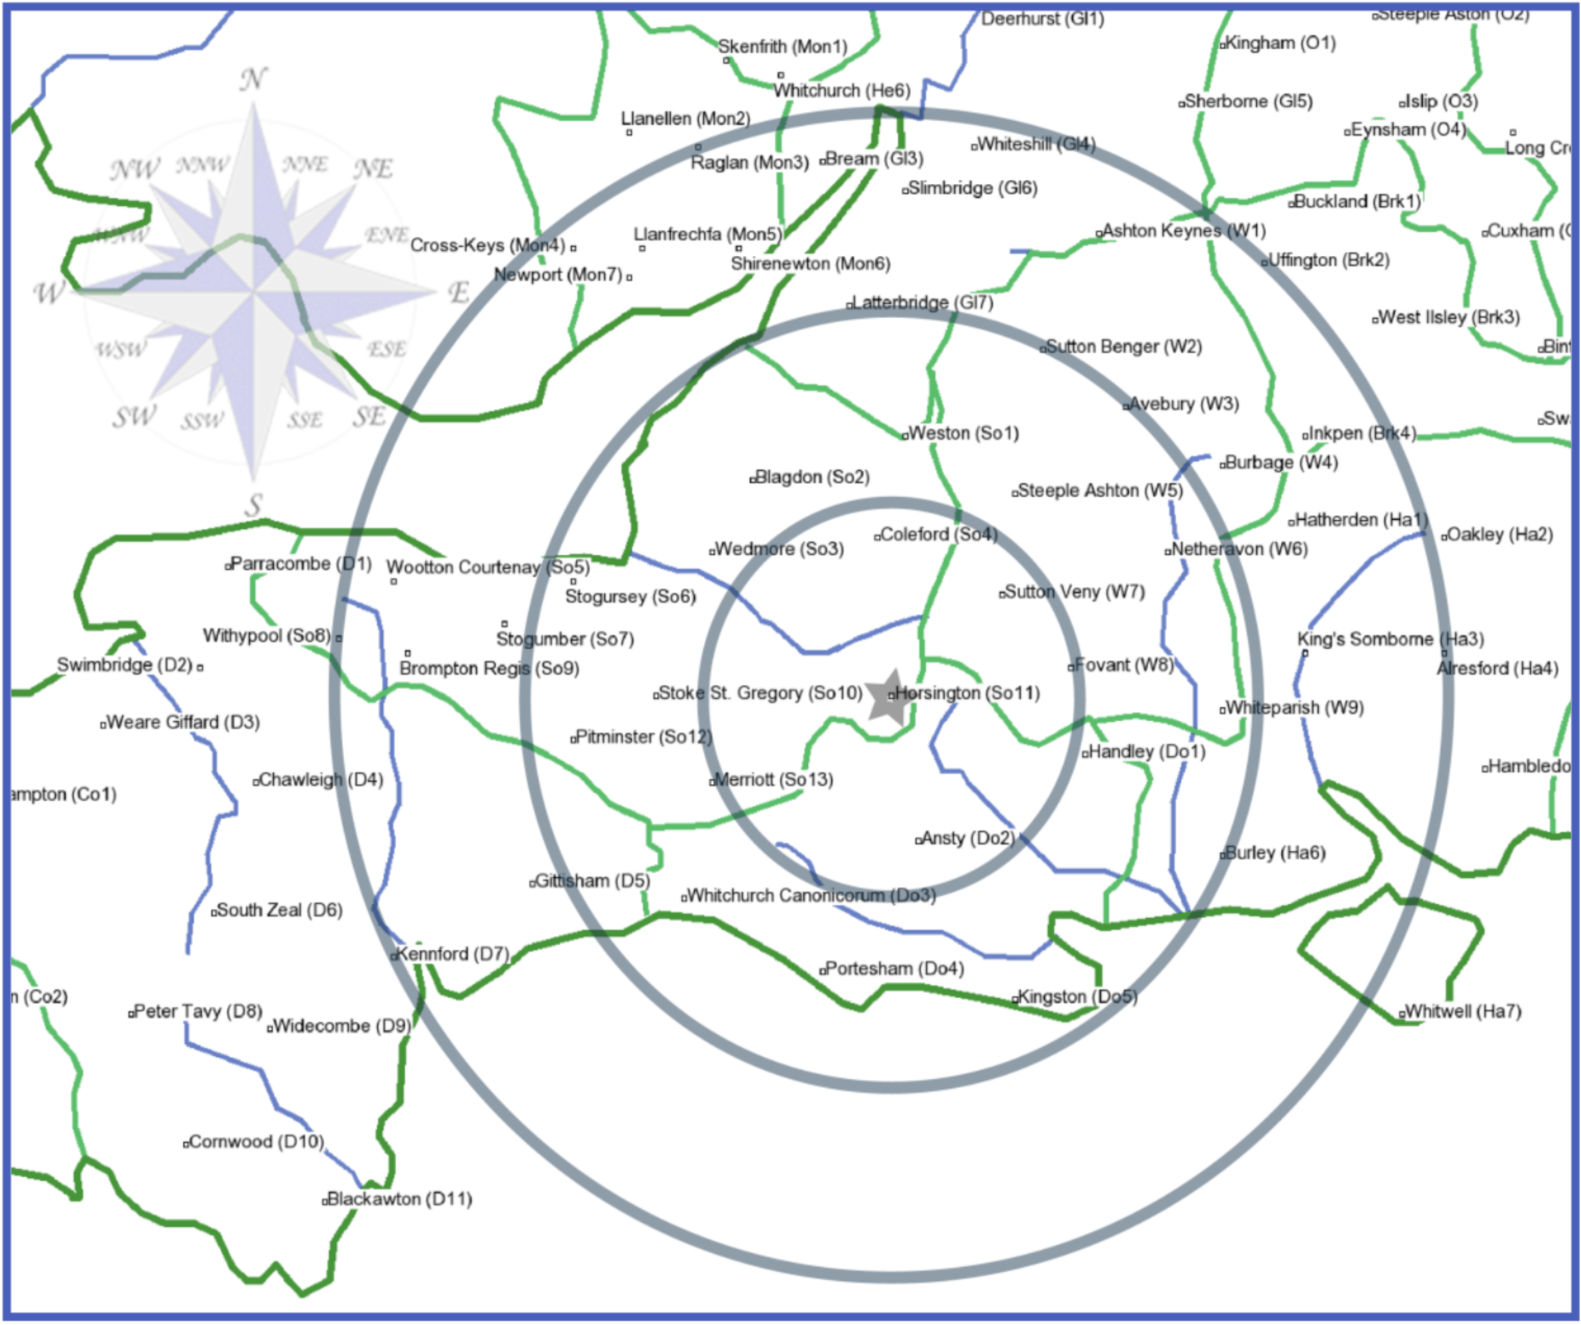
\includegraphics[width=\textwidth] {figures/ivdm6.pdf}
\addtocounter{figure}{-1}\renewcommand{\thefigure}{\arabic{figure}.11a}
% % % \captionsetup{name=Map}%
\caption {\textsc{ivdm6}: Distribution of putative input items from potential \textsc{sl} Horsington} 
\label{Map5.11a}
\end{figure}

The \isi{geo-linguistic distribution} of the putative input from Horsington's \textsc{sl} posed a challenge to my ``Blagdon core'' proposal. Like Blagdon the radius of its distribution is 81 km (3 cm), and its distribution seemed to encompass much of the same localities that are found within the area that makes up the west and south \isi{England} overlap that I refer to as the \textsc{wsw4}. Take a look at Horsington's \textsc{ccat} (\tabref{Table 5.7}) to get a better idea of the type of \isi{geo-linguistic distribution} that I was presented with.


\begin{table}
\begin{tabularx}{\textwidth}{lQ}
\lsptoprule 
\textbf{Concentric Circle 1} & \textbf{hear, broth, mouth, horse, woman, first, hog, hungry, fire} \\  
Stoke St. Gregory  (Somersetshire) & [jə\textsuperscript{ɽ}ː]  \\
Handly (Dorsetshire) &  [bɽɔf], [məʊf], [hɑsəz], [wʊmən]  \\
Sutton Veny (Wiltshire) &  [fəst], [hʌg]  \\
Wedmore (Somersetshire) &  [hɒgɽi]  \\
Blagdon (Somersetshire) &  [fɑɪə]  \\
\midrule\textbf{Concentric Circle 2} & \textbf{ask} \\
Latterbridge (Gloucestershire) &  [haks]\\
\midrule\textbf{Concentric Circle 3} & \textbf{four, care, iron, brother, eyes, hurt, finger, ears, hare, teeth, yesterday}\\ 
Llanfrechfa (Monmouthshire) & [fɔ], [kɛː], [əɪ-ɪn], [b\"ɑðə], [həɪz] \\
Newport (Monmouthshire) &  [hœːt], [fɪŋgə], [j\"œs] \\
Cross Keys (Monmouthshire) &  [heː\textsuperscript{ə}]\\
Brompton Regis (Somersetshire) & [tiːf] \\
Burbage (Wiltshire) & [estə\textsuperscript{ɽ}ɖeː] \\
\lspbottomrule 
\end{tabularx}
\caption{\textsc{ccat6}: Horsington (Somersetshire) \LSfrac{24/45} (21 variant to secure)}
\label{Table 5.7}
\end{table}

As can be seen from \textsc{ccat6} (\tabref{Table 5.7}) , Horsington's distribution includes seven of the same localities found in the Blagdon distribution, inclusive of Blagdon itself. These seven localities are Wedmore and Brompton Regis in Somersetshire County, Newport, Llanfrechfa and Cross Keys in Monmouthshire County, Latterbridge in Gloucestershire and Burbage in Wiltshire. The remaining localities, which are situated within one of the \textsc{wsw4} counties, or in a county neighbouring the \textsc{wsw4}, are Stoke St. Gregory, Sutton Veny and Handley, in Somersetshire County, Wiltshire County and Dorsetshire County, respectively. Let us take a closer look at the route that has to be taken from \textsc{sl} Horsington to the lects that provide the remaining input forms needed to complete the Sranan45 matches (see Figure \ref{Map5.11b}).


\begin{figure}
\includegraphics[width=\textwidth] {figures/ivrdm6.pdf}
\addtocounter{figure}{-1}\renewcommand{\thefigure}{\arabic{figure}.11b}
% % % \captionsetup{name=Map}%
\caption {ivrdm6: Distribution path of remaining input items from \textsc{sl} Horsington} 
\label{Map5.11b}
\end{figure}

Comparing \textsc{ivdm4} (Figure \ref{Map5.8a}) (Blagdon's distribution) with \textsc{ivdm6} (Figure \ref{Map5.11a}) (Horsington's distribution), we see where Horsington's \isi{geo-linguistic distribution} of the \isi{putative input etyma} poses a challenge to Blagdon's status as the core lect at the centre of the \textsc{wsw4} input for the Sranan45. This presented me with the following possibilities:

\begin{enumerate}
\item {Horsington is the core lect from which \isi{linguistic features} spread outwards, prior to dialect internal changes and these features became preserved in Blagdon. The problem with this possibility was that if I was to accept it, then I would also have to accept that the reverse was also possible; i.e. that Blagdon is the core lect from which the influence had spread prior to its undergoing internal linguistic changes.}
\item{Blagdon is the core lect but by virtue of Horsington being in such close geographic proximity, i.e. in the same county, the \isi{linguistic feature mapping} actually captured Blagdon's features from one of its closest geo-linguistic lects.}
\item{The input core is a Blagdon/Horsington composite.}
\end{enumerate}

Keeping possibilities two and three in mind, I refrained from drawing any conclusions and instead went on to look at the distribution from Wedmore, the third and final potential core \textsc{sl} for the south of \isi{England} (see Figure \ref{Map5.12}).

\begin{figure}
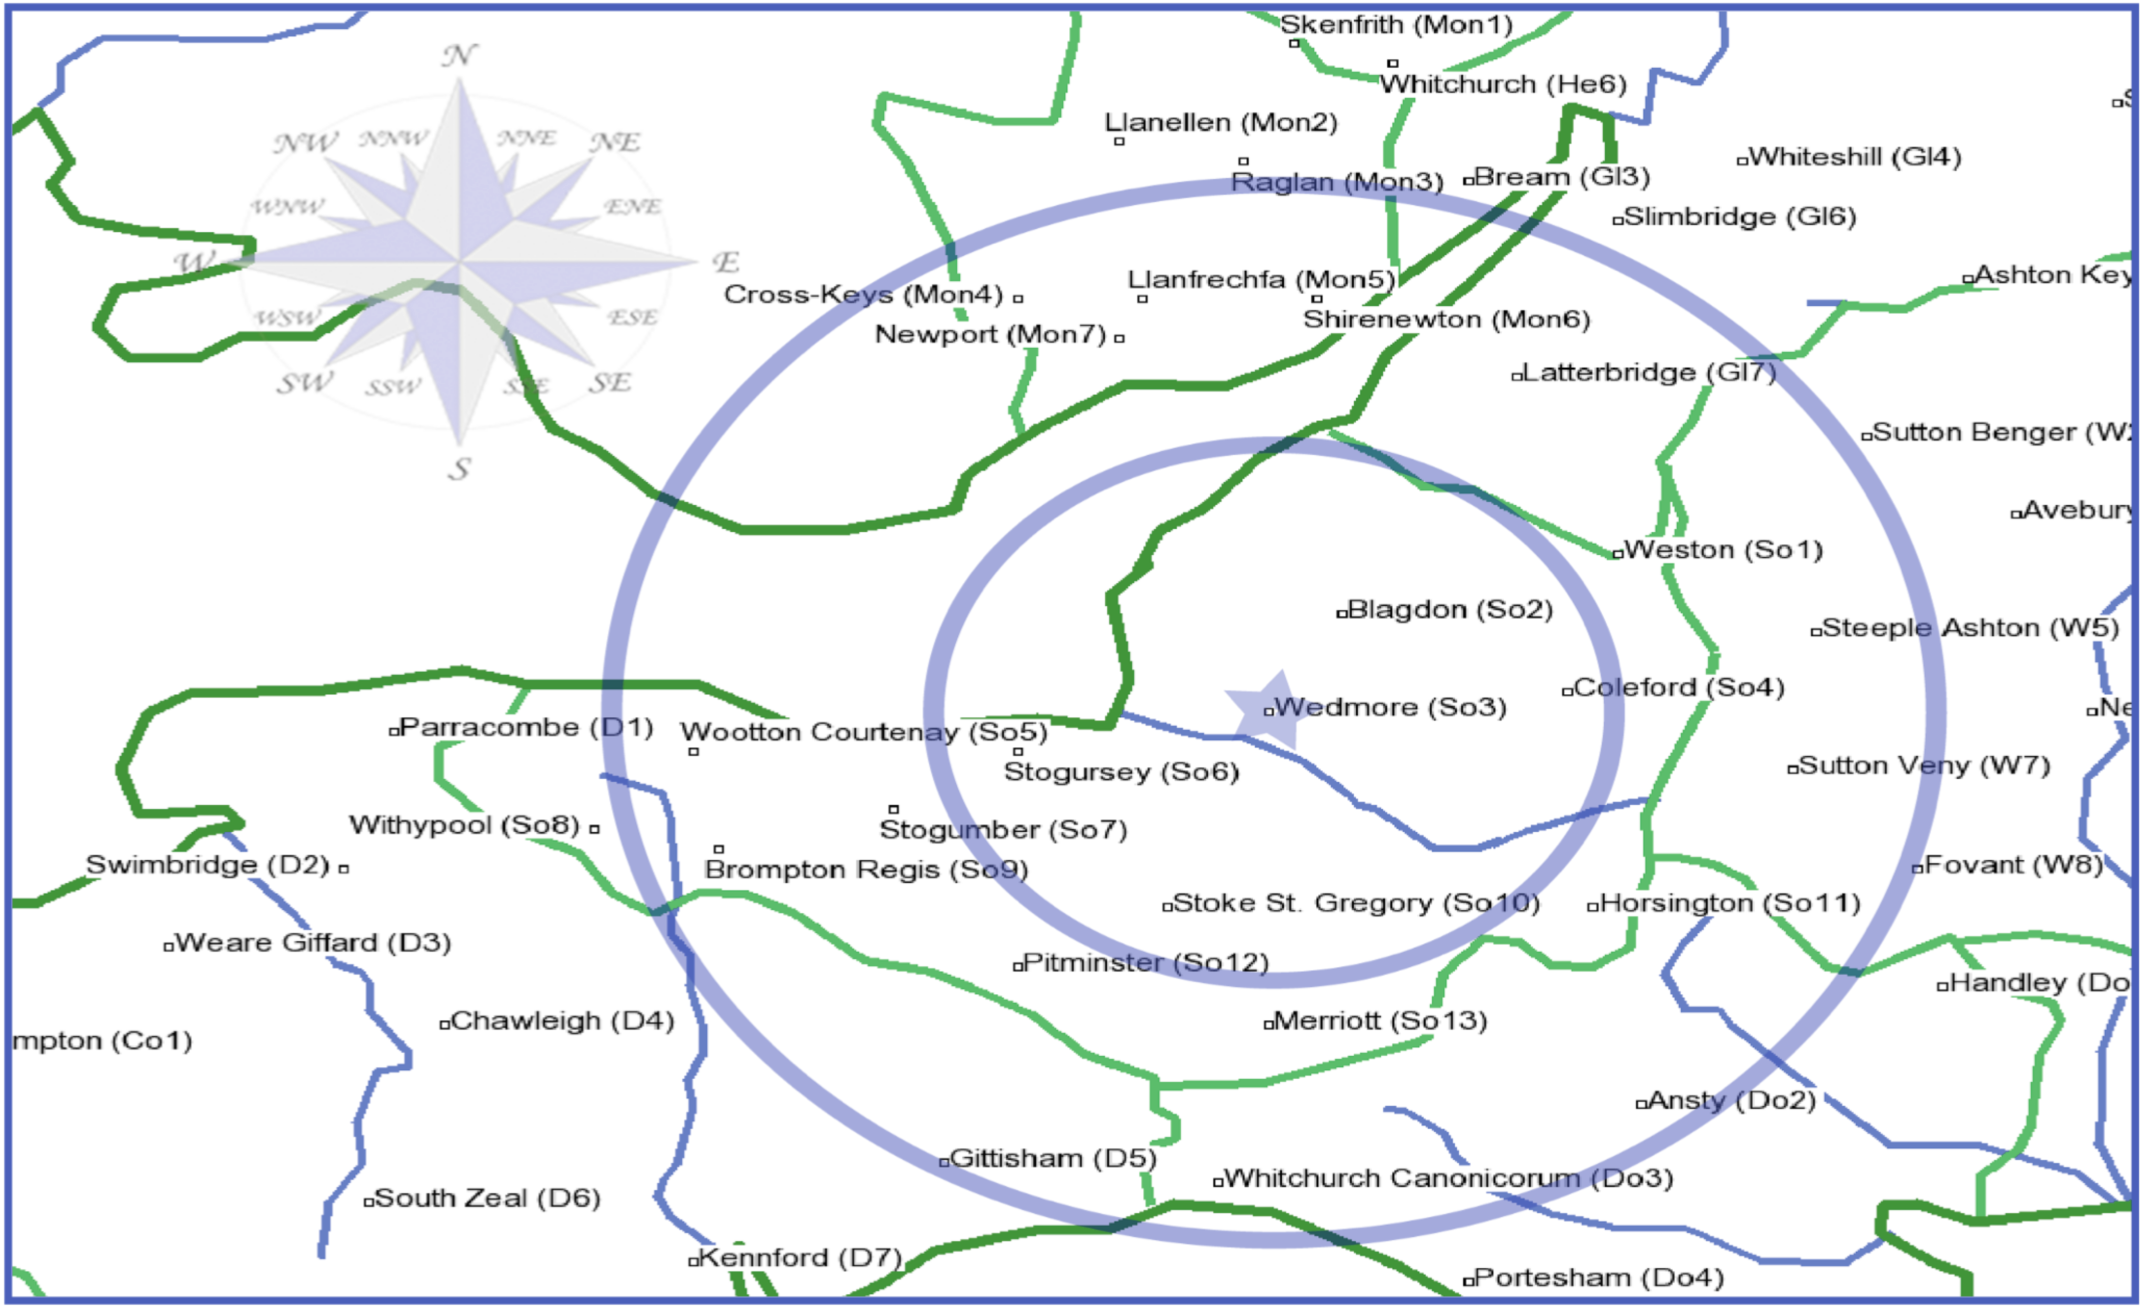
\includegraphics[width=\textwidth] {figures/ivdm7.pdf}
\addtocounter{figure}{-1}\renewcommand{\thefigure}{\arabic{figure}.12}
% % % \captionsetup{name=Map}%
\caption {\textsc{ivdm7}: Distribution of putative input items from potential \textsc{sl} Wedmore} 
\label{Map5.12}
\end{figure}

The \isi{geo-linguistic distribution} of the putative input items from \textsc{sl} Wedmore is more concentrated than noticed with Blagdon's and Horsington's. Wedmore, which is 6.75 km (0.25 cm) away from Blagdon and 11.34 km (0.42 cm) away from Horsington, boasts a 54 km (2 cm) radius in which all the \textsc{sed45} \isi{putative input etyma} for the \textsc{Sranan45} are secured. This is 27 km (1 cm) smaller and hence more concentrated than the Blagdon and the Horsington geo-linguistic clustering of the input etyma. Take a closer look at the \isi{locality-by-locality distribution} of these putative Sranan45 \textsc{sed} input etyma.


\begin{table}
\begin{tabularx}{\textwidth}{lQ}
\lsptoprule 
\textbf{Concentric Circle 1} & \textbf{woman, master (husband), mouth, horse, fire, hog, gutter, hear} \\  
Blagdon (Somersetshire) &  [wʊmən], [wʊmən], [mɛːstə\textsuperscript{ɽ}], [maʊθ], [hɑs], [hɑg]  \\
Coleford (Somersetshire) &  [gʌtəɽ]\\
\textbf{Concentric Circle 2} & \textbf{hare, hear, arse, ask, yesterday, hurt, finger, ears, four, care, iron, brother, eyes}\\
Weston (Somersetshire) &  [hɛː\textsuperscript{ə}], [jə\textsuperscript{ɽ}ː] \\
Horsington (Somersetshire) &  [a\textsuperscript{ɽ}ʂ] \\
Latterbridge (Gloucestershire) &  [haks], [estə\textsuperscript{ɽ}ɖe]\\
Newport (Monmouthshire) &  [hœːt], [fɪŋgə], [j\"œs] \\
Llanfrechfa (Monmouthshire) & [fɔ], [kɛː], [əɪ-ɪn], [b\"ɑðə], [həɪz] \\
Brompton Regis (Somersetshire) & [tiːf] \\
\lspbottomrule 
\end{tabularx}
\caption{\textsc{ccat7}: Wedmore (Somersetshire) \LSfrac{24/45} (21 variant to secure)}
\label{Table 5.8}
\end{table}

Except for Dorsetshire, situated to the immediate south of Somersetshire and Wiltshire, the distribution of the putative input items from \textsc{sl} Wedmore comprises of localities found within three of the four counties that make up the \textsc{wsw4}; these are Somersetshire, Monmouthshire, and Gloucestershire. In fact, this geo-linguistic area of distribution is observable at the heart of a Blagdon $\sim$ Horsington composite distribution area. This is illustrated in Figure \ref{Map5.13}.
  

\begin{figure}
\includegraphics[width=\textwidth] {figures/overlap-dist.pdf}
\addtocounter{figure}{-1}\renewcommand{\thefigure}{\arabic{figure}.13}
% % % \captionsetup{name=Map}%
\caption {Overlapping Geo-linguistic distributions: Wedmore, Horsington and Blagdon} 
\label{Map5.13}
\end{figure}

Figure \ref{Map5.13} shows the Wedmore area (coloured green), within which we can identify the putative input items, as being a subset of the composite of the Blagdon (coloured red) and Horsington (coloured purple), areas. I had, in light of this distribution, three major contenders for the core lect of influence at the centre of the putative \textsc{wsw4} \isi{regional input} of origin for the Sranan45. First is Blagdon, which exhibits an 81 km (3 cm). Second is Horsington, which like Blagdon exhibits an 81 km (3 cm) long radius, geo-linguistic concentration of the \isi{putative input etyma}, albeit with a three-locality difference in which some of the putative input items are secured. There is no Coleford (Somersetshire) in the \isi{geo-linguistic distribution} of the putative input from potential \textsc{sl} Horsington, and there is no Handley (Dorsetshire) and Sutton Veny (Wiltshire) in the distribution from Blagdon. Third is Wedmore, with the most concentrated \isi{geo-linguistic distribution} of the \isi{putative input etyma} for the Sranan45; i.e. all the putative input is found within a 54km (2 cm) radius in all directions from this core lect. I contemplated for a while on whether I was to:

\begin{enumerate}
\item {Accept Blagdon's status as core \isi{input dialect}, based on the \isi{statistics} presented in \chapref{ch:4}, alongside its concentrated distribution of the \isi{putative input etyma} presented in this chapter.}
\item{Relinquish and/or share its status of core lect of input with Horsington and Wedmore.}
\item{Abandon the Blagdon \isi{statistics} and/or the geo-linguistic similarities between Blagdon and Horsington in favour of a Wedmore core, given the `most concentrated distribution' criteria, i.e. the area with the smallest radius of distribution being acknowledged as the input area.}
\end{enumerate}

Given that all three localities, i.e. Wedmore, Blagdon and Horsington, are situated within the county of Somersetshire, in close proximity to each other, I wondered whether regular linguistic diffusion might have been taking place across each of the three localities. I decided to break the impasse by selecting, at the heart of the \textsc{wsw4}, Blagdon-Horsington-Wedmore composite input that would serve as the core lect at the centre of the regional \isi{dialectal input} for the Sranan45. However, for this to be accepted, I needed to address one other issue. This issue involved the requirement to move to the localities Llanfrechfa (Monmouthshire) and Latterbridge (Gloucestershire) irrespective of the \textsc{sl}. Located in this general area, in close proximity to three of the \textsc{wsw4} counties, is Bristol, a city and port, whose importance will become more evident in \chapref{ch:6}.

Bristol, the city and port in the south of \isi{England}, borders Somersetshire and Gloucestershire to its immediate southwest and northwest, respectively. To the direct north, across the Bristol Channel, is the county of Monmouthshire. I discuss in \chapref{ch:6} the fact that this city-port played an integral role in the populating of the \ili{English} New World colonies, during the period in which \isi{Suriname} was settled by the \ili{English} and then subsequently ceded to the \ili{Dutch}, i.e. from 1650--1667.

Given the location of Bristol and its importance as a city-port during the relevant time in question, i.e. between 1650 and 1667, I asked myself the following question: ``Could it be that the localities in close proximity to Bristol, in any direction, best explained the source of influence in \ili{Sranan}?'' If this were true, then I would have a possible means by which to explain the high degree of correspondence observed between the four statistically significant localities in the south of \isi{England}, i.e. Blagdon, Wedmore, Horsington and Whitwell, and the Sranan45 reflexes. Two possible scenarios came to mind. Either Bristol was the core lect of influence from which the surrounding communities took and preserved various \isi{linguistic features}; or, the city-port was a melting pot of linguistic ingredients coming from the surrounding farming communities. I needed to look at what the \isi{geo-linguistic distribution} of the putative input items would look like if we began from Bristol, to see what light might have been shed on this matter (see Figure \ref{Map5.14}).

\begin{figure}
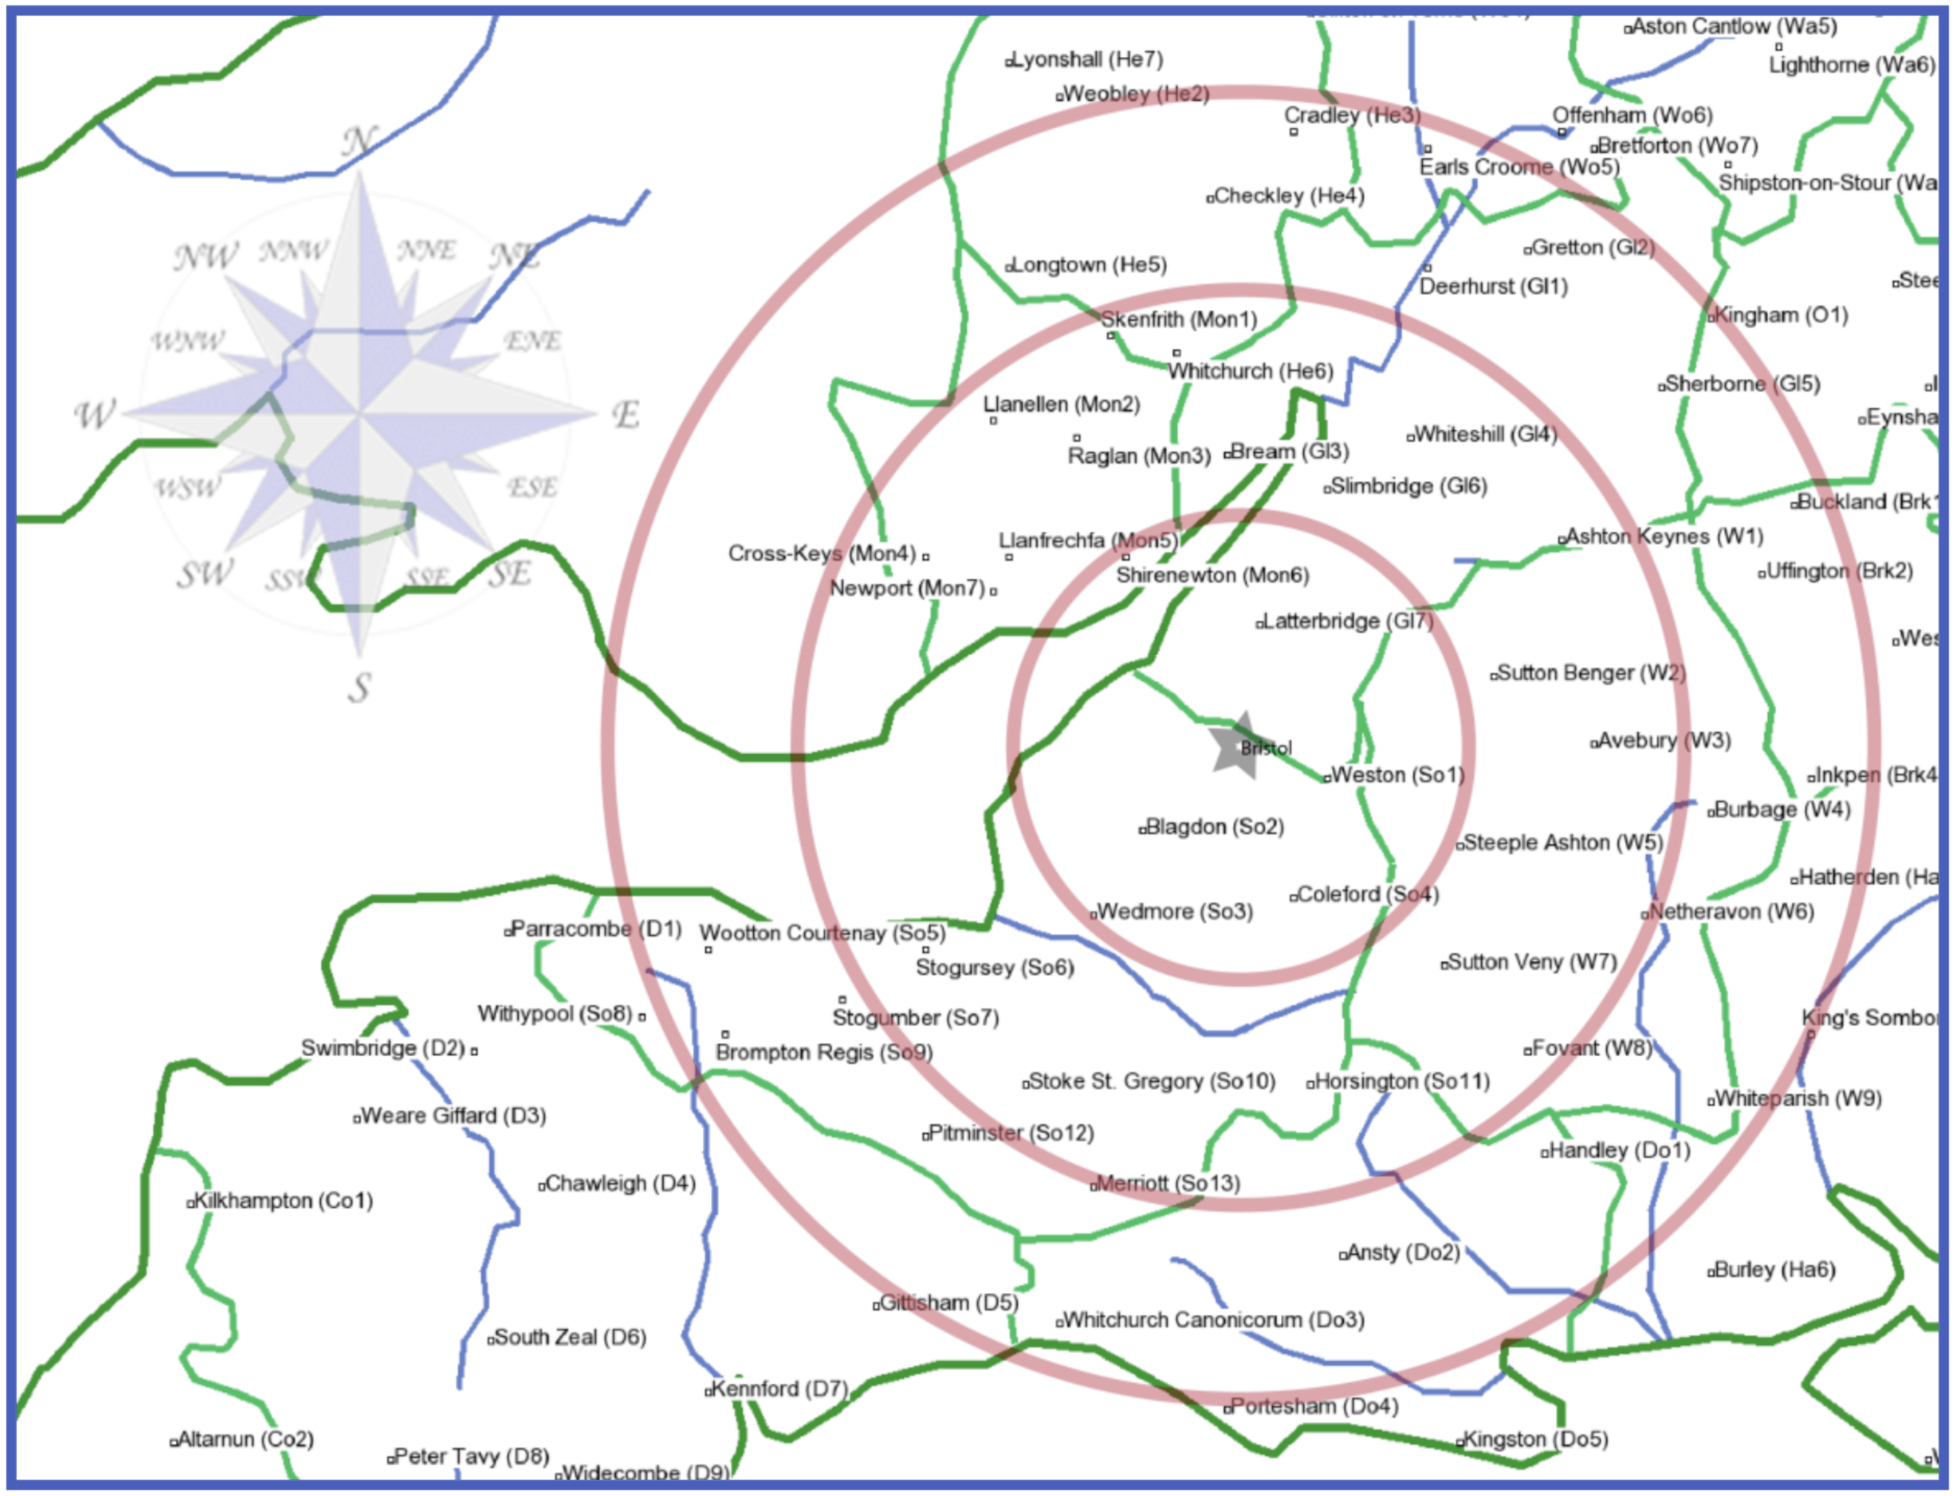
\includegraphics[width=\textwidth] {figures/ivdm8.pdf}
\addtocounter{figure}{-1}\renewcommand{\thefigure}{\arabic{figure}.14}
% % % \captionsetup{name=Map}%
\caption {\textsc{ivdm8}: Distribution of putative input items from potential \textsc{sl} Bristol} 
\label{Map5.14}
\end{figure}

\textsc{ivdm8} (Figure \ref{Map5.14}) highlights a distribution of the putative input that seems to comprise of the same localities observed in the distributions noticed from Blagdon, Horsington and Wedmore, inclusive of the three localities themselves; this distribution does not involve Whitwell, though it does include some portions of the Western end of the county of Hampshire. Take a look at the locality-by-locality breakdown to get a good idea of what type of distribution we are dealing with.

\begin{table}
\begin{tabularx}{\textwidth}{lQ}
\lsptoprule 
\textbf{Concentric Circle 1} & \textbf{arse, ask, yesterday, fire, hog, first, hand, head, help, house, master (husband), mouth, burn, cold, corn, curse, door, gold, hear, herring, horse, more (quantity), more, old, star, turn, woman, wear, work (noun), work (verb), gutter, broth, hungry, hot, remember} \\  
Latterbridge (Gloucestershire) &  [aɹs], [haks], [ɪstə\textsuperscript{ɽ}ɖɪ]\\
Blagdon (Somersetshire)        &  [fɑiə], [hɔg], [fɒst], [hænd], [hɛd], [hɛlp], [haʊs], [mestə\textsuperscript{ɽ}], [maʊf],
                                  [bə\textsuperscript{ɽ}ːn], [koʊld], [ka\textsuperscript{ɽ}ːn], [kɒs], [dɔ\textsuperscript{ɽ}], [goʊld],
                                  [jə\textsuperscript{ɽ}], [hə{ɽ}ɪn],  [hʌs], [mɔ\textsuperscript{ɽ}ː], [mɔ\textsuperscript{ɽ}], [oʊl],
                                  [sta\textsuperscript{r}ː], [tə\textsuperscript{r}ːn], [wʊmən],[wɛ\textsuperscript{ɽ}], [wə\textsuperscript{ɽ}k], 
                                  [wə\textsuperscript{ɽ}k]\\
Coleford (Somersetshire)        & [gʌtəɽ]\\
Wedmore (Somersetshire)         & [bɽɔːf], [hɒgɽi], [hɔt], [ɽɪmɛmbə\textsuperscript{ɽ}]  \\
\textbf{Concentric Circle 2}    & \textbf{brother, eye, ears, four, care, hurt, iron, finger, hear}\\
Llanfrechfa (Monmouthshire)     & [b\"ɑðə], [həɪ], [j\"œs], [fɔ], [kɛː], [hœːt], [əɪ-ɪn]   \\
Newport (Monmouthshire)         & [fɪŋgə] \\
Cross Keys (Monmouthshire)      & [heː\textsuperscript{ə}]\\
\textbf{Concentric Circle 3}    & \textbf{teeth}\\ 
Handley (Dorset)                & [tiːf] \\
\lspbottomrule 
\end{tabularx}
\caption{\textsc{ccat8}: Bristol \textsuperscript{x}\LSfrac{/45} (45 variants to secure)}
\label{Table 5.9}
\end{table}

Similar to the \isi{geo-linguistic distribution} of the putative input from Blagdon and Horsington, Bristol boasts an 81 km (3 cm) radius in which all input etyma are secured. This provides competition for the Blagdon-Horsington-Wedmore composite \isi{input lect} proposal. Barring Dorsetshire, the localities observed within the distribution of the input items from Bristol, are situated in three of the four \textsc{wsw4} counties, i.e. Somersetshire, Gloucestershire and Monmouthshire. Blagdon, the locality of highest correspondence to the Sranan45 and Wedmore, the locality with the most concentrated distribution of the putative input, are found within this distribution. However, the greatest number of the Sranan45 \ili{English} etyma is observed in Blagdon (see \textsc{ccat8} (\tabref{Table 5.9})).

The \textsc{sed} did not cover urban areas and therefore excluded Bristol. Consequently, it was not possible to determine whether in the time of the \textsc{sed} survey, the Bristol linguistic forms could have provided a perfect match for the 45 putative input needed for the Sranan45. However, it is clear that the port and the localities within the surrounding counties, specifically those in Somersetshire and others within and around the remaining \textsc{wsw4} counties, contributed significantly to the \ili{Sranan} input (see Figure~\ref{Map5.15}). This is because all relevant lexical and phonetic and idiosyncratic lexical and phonetic \isi{linguistic input} forms are found within a dense \textsc{wsw4} concentration of localities that are within close proximity to Bristol.

\begin{figure}
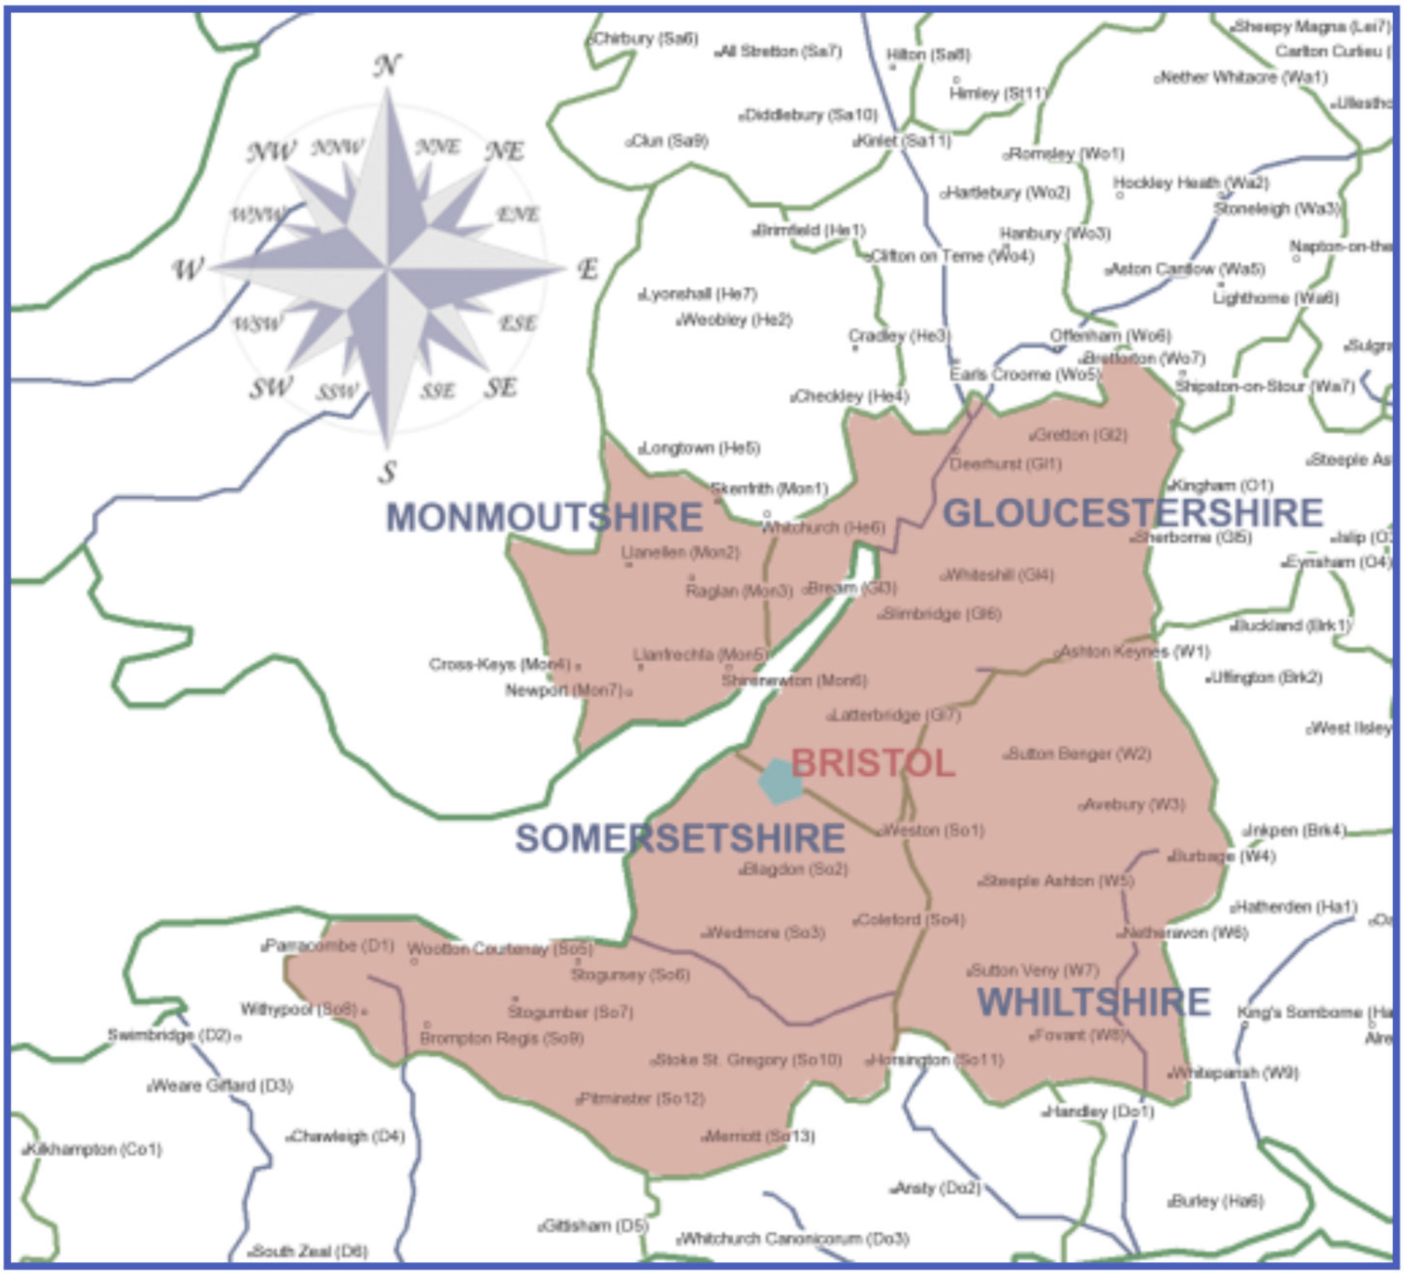
\includegraphics[width=\textwidth] {figures/wsw4.pdf}
\addtocounter{figure}{-1}\renewcommand{\thefigure}{\arabic{figure}.15}
% % % \captionsetup{name=Map}%
\caption {The \textsc{wsw4} counties in proximity to the port of Bristol}
\label{Map5.15} 
\end{figure}

\section{Summary of findings and the way forward}
Whether I began from \textsc{sl} Wearhead in the north of \isi{England}, or \textsc{sl} Canewdon in the east of \isi{England}, there was need to go to localities within the \textsc{wsw4} to secure various idiosyncratic items specific to that region. There was a move specifically to localities Latterbridge, Newport and Llanfrechfa, which are the only lects in which three peculiar items were observed; i.e. \emph{ask} [haks] with word-initial [h] and +\textsc{ccr} /sk/ $\rightarrow$ [ks], \emph{eye} [həɪ] with word initial [h] and \emph{ears} [j\"œs] with +Pal., respectively.

When, on the other hand, I began from the \textsc{sl}s Earl's Croome and Blagdon, in the west and south of \isi{England} respectively, there was no need to go anywhere outside of the \textsc{wsw4} to secure any of the \isi{potential input} etyma for the Sranan45. This \textsc{wsw4} \isi{England} concentration of acceptable input etyma for the Sranan45 therefore represented strong evidence against an ``all-over'' \isi{England} account of origin. As it concerns the issue raised regarding whether there was any denser distribution of the input than noticed from Blagdon, the answer is yes, since the distribution from Wedmore provided this denser distribution. Notwithstanding, Wedmore formed part of a composite core lect, alongside Horsington and Blagdon (all in Somersetshire county) that formed the central core of a \textsc{wsw4} region of input; this region includes the counties Somersetshire, Wiltshire, Monmouthshire and Gloucester. The \isi{dialect geography} tool did not, however, account for the three statistically significant East Anglian localities of Canewdon, Doddinghurst and East Mersea. I still needed to explain these three lects. These results led to two questions that the third component of my methodological tool would need to answer. The first is as follows:

\begin{quote}
\emph{``Do we have historical evidence of migration from the \textsc{wsw4} and its neighbouring counties, going to \isi{Suriname}, via Bristol and/or from any other port, within the period 1650--1667?''}
\end{quote}

If the answer to the above question were in the affirmative, this would represent corroboration of the results of the \isi{statistics} and the linguistic \isi{geography}, thereby providing strong evidence for a \textsc{wsw4} input. The second question is as follows:

\begin{quote}
\emph{``Do we have historical evidence of migration from any nearby port in the east and East Anglia localities of \isi{England}, going to \isi{Suriname} within the period 1650--1667?''}
\end{quote}

The answer to this question, if in the affirmative, would provide support for that part of the results of the statistical analysis that presented three statistical probable East Anglian input lects for the Sranan45. These questions and more are addressed in \chapref{ch:6}, \emph{The Historical Complement}.
